\chapter{Demystifying Neurodivergence via Score Estimators }
\label{ch:demyst}

Given the success of MSMA for anomaly detection on benchmark experiments, we will now explore whether this methodology allows for any new \textit{scientific} insights.
Assuming the underlying model has learned rich information about the data, can it help us uncover useful knowledge about our dataset? I will try to answer that question by focusing on a narrow task: detecting neuroatypicalities from structural MRIs of pre-pubertal brains.
% The task was chosen such that \textit{if} a novel insight is derived, it may be of direct use to the medical research community.

% Developmental disorders leading to atypical brain development are commonly diagnosed in children through clinical assessments that measure behavioral response. While effective in diagnosis, behavioral assessments do not provide any insight into the differences in brain morphometry of the neurodivergent cohort.
Neurodevelopmental disorders are disabilities associated primarily with the functioning of the brain. Certain disorders such as Down Syndrome, Fragile-X Syndrome and Angelman Syndrome can be detected via genetic testing. Others, such as Autism Spectrum Disorder (ASD) and Attention-Deficit/Hyperactivity Disorder (ADHD), are diagnosed through clinical assessments that measure behavioral response. While effective in diagnosis, neither genetic testing nor behavioral assessments provide insight into the differences in \textit{brain morphometry} of the neurodivergent cohort. Furthermore, there is evidence for a heterogeneity in the underlying brain structures for certain brain disorders, such as ASD~\cite{heteroasd}. This implies that the same behavior can be originated from different atypical brain development.

Existing analyses primarily look at group wise differences of brain features (such as region volumes) between cohorts~\cite{giraultNeurodevelopmentAutismInfancy2020,hamnerPediatricBrainDevelopment2018}, or correlations of said features with a behavioral assessment~\cite{shenSubcorticalBrainDevelopment2022,brainsci12040439}.
% These analyses fail to produce specific causal relationships between the brain regions and the neurodivergence, as they mainly focus on correlational evidence.
These analyses forgo a broad study of all brain regions in favor of specific regions that are more relevant to the disorder. This is an understandable trade-off as reserarchers often have strong prior evidence that correlates brain regions to behavioral actions, and have limited time and resources. However, in making this trade-off, these analyses are less likely to uncover novel associations between brain regions and behavioral phenotypes (in the context of the neurodevelopmental disorder).
Furthermore, the researchers introduce additional biases when they select regions of interest (ROIs) to be studied using their preconceived notions about the disorder.

Herein lies the opportunity for a data-driven methodology to uncover atypically developing ROIs that are reflected in the data but, may be underexplored in the existing  literature. One can task a model to identify subgroups that deviate from the typical (via outlier detection), and subsequently highlight the brain morphometry shared across the subpopulations (via localization).  MSMA, combined with its localization augmentation, naturally allows for such data exploration. This chapter outlines a process through which MSMA was utilized to derive insights about brain MRI data.

\section{A Hypothesis Generating Tool}

The previous chapters have demonstrated MSMA's anomaly detection capabilities. At the heart of MSMA is the score-norm vector. These vectors describe a space in which the outliers become separable from the inliers. How can one explore this space to gain further insights into the data?

We can assume that a user exploring the outputs of MSMA will be looking to answer a set of research questions. Examples of the questions may be:
\begin{itemize}
    \item Do any atypical subpopulations cluster in the score-norm space?
    \item Can we identify atypical input features (such as brain ROIs)  that are shared among samples within a cluster?
    \item Do atypical subpopulations in the score-norm space correlate with any non-morphometric measurements (such as behavioral assessments)?
\end{itemize}

To answer such questions, one needs to be able to link multiple sources of data: the score-norm space, the localization heatmaps, and existing metadata associated with each sample. I posit to use an interactive visualization to facilitate such a task.
Using this visualization the user should be able to observe how samples are distributed/clustered in the score-norm space. Additional views can show the aggregated localization heatmaps for each cluster, as well as metadata such as behavioural scores.

% The visualization will also display an aggregate of anomaly scores across brain ROIs. The goal of the visualization is to make the results interpretable by a medically informed audience. By using standardized brain parcellation schemes, the visualization should enable the user to identify the most anomalous ROIs for the population of interest, and refer to the medical literature for further analysis.

\section{Exploring a High-Dimensional Space}

It is often desirable to visualize data for the purposes of exploratory research. This poses a problem if we want to visualize the space of score-norms (as a 2D image). While the score-norms are much lower in dimensionality compared to the high resolution MRIs they are derived from, each score-norm vector is still multidimensional. For reference, all of the experiments in this chapter use $L=20$ scales, resulting in a 20-dimensional vector for each sample. One has to utilize a dimensionality reduction algorithm to reduce the space into two or three dimensions so that the points may be visualized on a screen.

This section will briefly go over existing dimensionality reduction algorithms and why they may not be appropriate for our analysis as they can introduce spurious clusters in the visualization. Instead, I will be advocating the use of Self-Organizing Maps (SOM)~\cite{kohonen1990self}  to visualize my data and will discuss its advantages.


\subsection*{Common Dimensionality Reduction Algorithms}

Most commonly, researchers have used Principal Component Analysis (PCA)~\cite{abdi2010principal}) to select the most important components in the data. PCA finds the eigenvectors of the correlation matrix of the data. Intuitively, these eigenvectors capture the largest variation in the data. While this technique is fast and well understood, it has the downside of only capturing \textit{linear} subspaces as it will select orthogonal components of increasing variation. Therefore, it is most effective for visualization when the data itself is linearly separable. Recently, two other techniques have gained popularity as methods to visualize high dimensional non linear data: t-SNE and UMAP.  

% \subsection*{A Brief Discussion on t-SNE and UMAP}

t-SNE (t-distributed Stochastic Neighbor Embeddings) defines the relative distance between two points as a conditional probability. It uses an optimization process to determine a low-dimensional embedding such that the relative distance between each point in the low-dimensional space matches the distance in the high-dimensional space (using the Kullback-Leibler Divergence between the pairwise conditional probability distribution).

UMAP (Uniform Manifold Approximation and Projection) computes the low-dimensional embedding in two stages. First, it constructs a weighted graph of the k-nearest neighbours (the number of neighbors being a hyperparameter). The weights of the graphs represent probability distributions. In the second stage, it uses an iterative procedure to pull the neighbors in the graph closer together in the low-dimensional space. Additionally, it applies a repulsive force between all non-neighbours in the graph, pushing them away in the low-dimensional space. Generally, UMAP is considered to have superior runtime performance compared to t-SNE~\cite{mcinnes2020umap}

% \subsection*{t-SNE and UMAP Need Not Reflect the Data}
\subsection*{t-SNE and UMAP Do Not Reflect True Distances}

% why are they not optimal for the task?

Both t-SNE and UMAP aim to find a low-dimensional space that reflects the distances in the original space. However, the resulting low-dimensional space is highly dependant on the hyperparameters. These hyperparameters (associated with the size of the neighbourhood considered) produce a trade-off between the preservation of local structure and preservation of global structure. Often, the algorithms are unable to preserve both~\cite{pacmap}. If local structure is emphasized, the algorithms produce spurious clusters, making their results untrustworthy. Conversely, if global structure is emphasized, the algorithms tend to produce large homogenous blobs, and fail to distinguish any underlying patterns~\cite{leiQuantifyingImpactUninformative2023}.
% This can have the unfortunate effect of the practitioner tweaking the hyperparameters until the algorithm's output plots that coincide with the practitioner's existing beliefs.


\subsection*{Self Organizing Maps as an Alternative}

The Self-Organizing Map, also known as Kohonen Networks, ~\cite{kohonen1990self} produces a two-dimensional grid-like map such that each cell on the map corresponds to a location in the data-space. Nearby cell locations on the grid are closer in the data-space compared to distal cell locations. A cell is commonly also referred to as a 'neuron'.

During training, the method randomly initializes a grid of neurons (cells). Note that the weight vector corresponding to each neuron resides in the data-space. For each data sample we find the closest neuron to the current point. This is referred to as the Best Matching Unit (BMU). The BMU's weights are updated to be closer to the data point. Additionally, the neighboring neurons (in the \textit{grid-space}) are also updated. The latter step is crucial to preserve the topological structure of the data. This procedure is repeated for a pre-defined number of iterations. Most online packages implement the batch-learning algorithm described by~\cite{kinouchi2002quick}. The authors improve convergence by initializing the neurons using the first two eigenvectors computed from the data, and by modifying learning objective to use the full dataset in each weight update rather than a minibatch as in the original algorithm.  I will be using the latter training algorithm.

\subsection*{SOMs Circumvent Dimensionality Reduction}

Note that SOMs operate directly in the high-dimensional data space, computing distances between the data points and the neuron prototypes in this original space. The topological constraint on the grid of neurons mainly facilitates the visual organization. This is in contrast to t-SNE and UMAP, which first project the data into a low-dimensional space, where distance computations may not accurately reflect the true distances in the high-dimensional space. As a result, SOMs can better preserve the structure and relationships within the data, reducing the risk of distortions introduced by dimensionality reduction.

\subsection*{SOMs Identify Prototypes}
It is helpful to think of SOM as a vector quantization algorithm with a spatial constraint on the codebook of vectors. Thus, each neuron can be interpreted as a prototype in the data-space. The grid-like structure of SOMs provides a natural way to organize these data prototypes. The relative positions of the neurons on the grid reflect their similarities. This spatial organization can aid in identifying patterns, clusters, or relationships within the data that may not be immediately apparent from a scatter plot produced by techniques like t-SNE or UMAP.

To elucidate how one can use SOM to gain insights about the data, recall that each sample is assigned to a single neuron (the sample's BMU). If class labels are available, we can tally up the labels of all the samples that are assigned to a given neuron. The maximally matching label can then be computed for each neuron. This label is often overlayed on top of the map visualization to quickly associate the prototype with a population. ~\figref{fig:som-cifar} shows an example of a SOM trained on the CIFAR-10 score-norms. Overlayed are examples of prototypical BMUs for OOD datasets. The BMUs displayed are those that matched at least 1\% of the samples belonging to the OOD dataset. Note the spread of certain datasets such as SVHN.

\begin{figure}[tbhp]
\centering
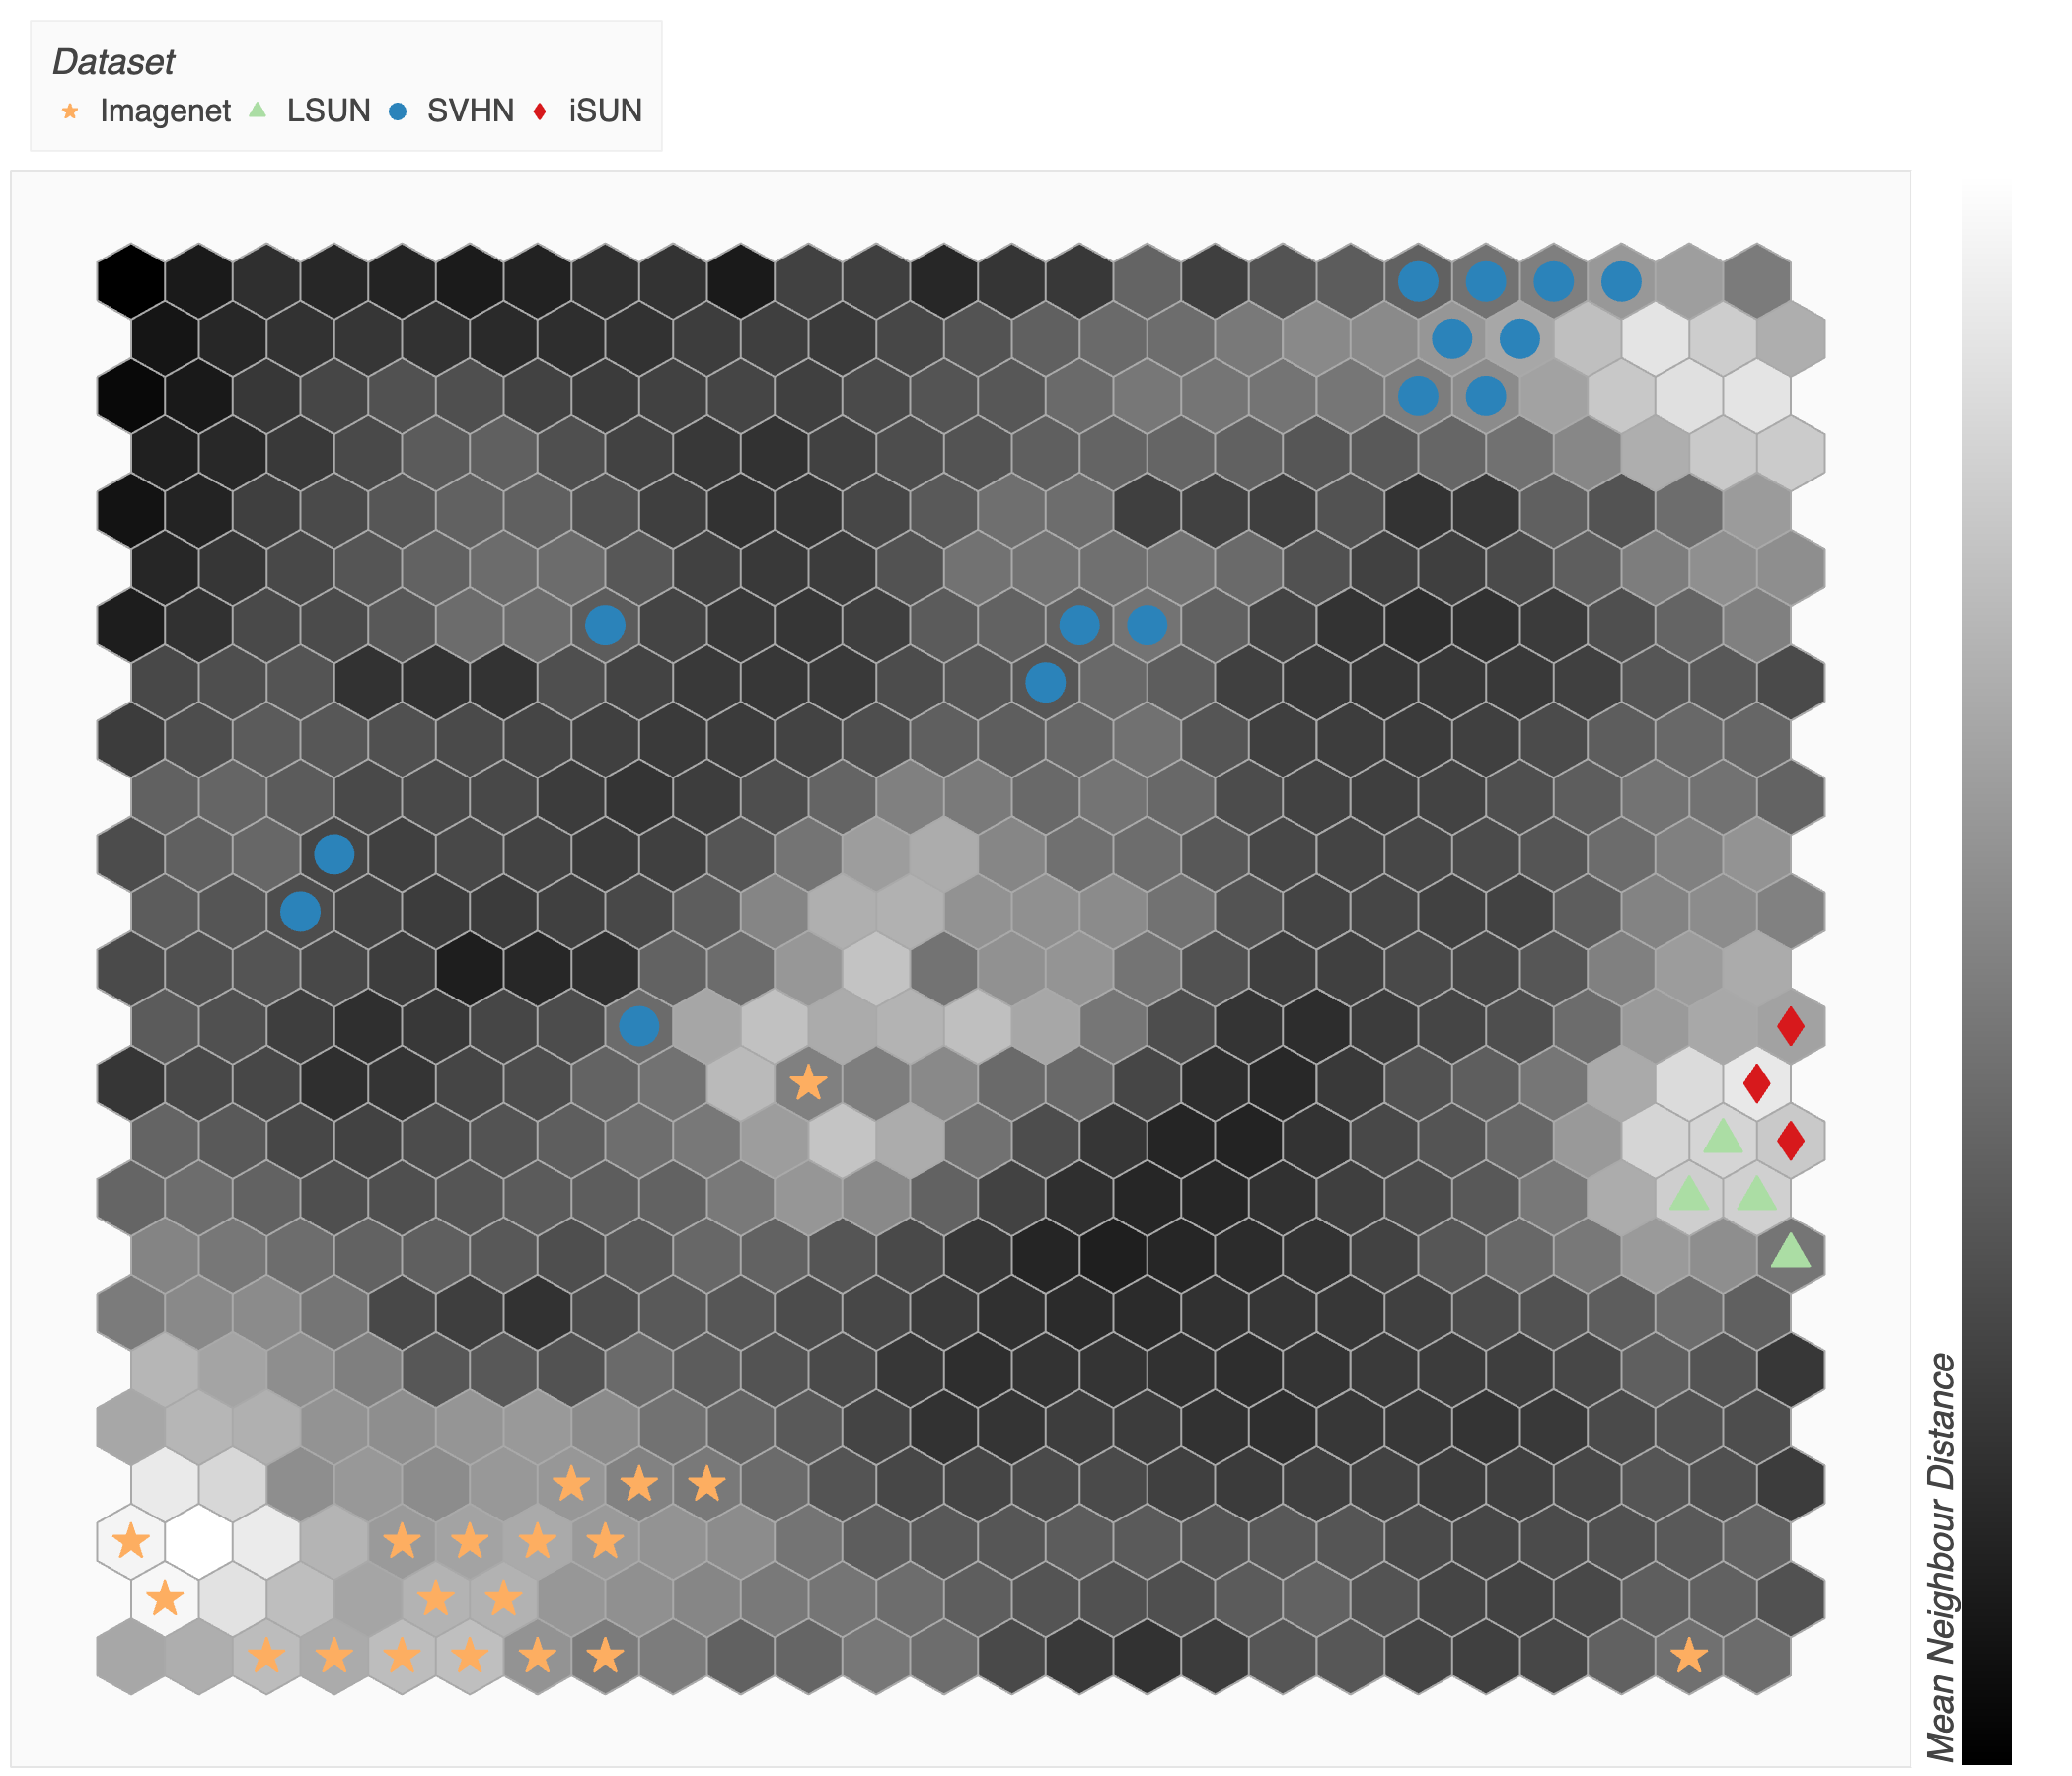
\includegraphics[width=\textwidth]{figures/cifar_som_hex.png}
\caption{A 25x25 SOM trained on the score-norms of CIFAR-10. Overlayed are examples of BMUs belonging to OOD data.}
\label{fig:som-cifar}
\end{figure}



% One can go further and analyze the hsitogram
% \subsection*{SOM vs tsne for clustering}

% \section{Feasibility Experiments on Benchmark Datasets }

\section{Case Study: Detecting Brain Regions involved in Down Syndrome}

This case study will explore how MSMA can be used to derive scientific insights. We will focus our analysis on a particular neurodevelopmental disorder: Down Syndrome. 

% Choosing a disorder that is relatively well understood allows us to ground our discoveries by comparing to the literature 

Down Syndrome (DS) is one of the most common neurodevelopmental disorder, occurring at a rate of ~1/700 live births~\cite{parker2010updated}. Studies have revealed large deviations from typical development in brain structure of children with DS, with the most pronounced deviation in the total brain volume (TBV). Further, when TBV is accounted for, studies have revealed deviations in specific regions of the brain such as the temporal lobe, cerebellum, and hippocampus~\cite{hamnerPediatricBrainDevelopment2018}. However, there remains a push for developing focused research to elucidate the nature of DS neuroanatomic phenotypes~\cite{hamnerPediatricBrainDevelopment2018}. While individuals with DS present with a rather heterogeneous set of behavioral and cognitive challenges, existing neuroimaging studies investigate atypical brain morphometry in DS from the viewpoint of a single, homogeneous population.

This case study aims to uncover brain morphometric phenotypes that are associated with DS, using learned score-estimates. It will incorporate MSMA, SOMs, and Spatial-MSMA to provide a cohesive analysis of structural brain MRIs belonging to a DS cohort. We will be answering the following research questions:

\begin{itemize}
    \item Does the score-norm space produced by MSMA \textit{cluster} any atypical neuroanatomic phenotype(s) pertinent to DS?
    
    \item Can Spatial-MSMA \textit{isolate} brain regions relevant to the phenotype?
    
    \item Do the regional anomaly scores \textit{correlate} with any behavior assessment?
\end{itemize}


    % - Can Spatial-MSMA isolate brain ROIs relevant to the prototype?

	% - Does Spatial-MSMA highlight brain ROIs that are \textit{known} in the existing research?

	% - Does Spatial-MSMA highlight brain ROIs that are \textit{novel}?

\subsection*{Data and Methodology}
 % As a first pass, all images with low automated QC scores were removed. --- > move this into appendix or ch:local
 
As in Chapter~\ref{ch:localizing}, we will be using samples from the ABCD and HCPD study as our reference inliers. I will denote this as ABCD-HCPD. This cohort was preprocessed to remove any outlying samples. To keep the inlier cohort as nominal as possible, we used the Child Behavior Checklist (CBCL)~\cite{achenbachChildBehaviorChecklist1999} scores as our filtering mechanism. This checklist assesses the behavior and emotional competencies of children. Children with behavioral problems tend to score high on this test. For our analysis, all children that scored above a t-score of 66 ($\tilde{95}$-th percentile) in the summary scores as well as \textit{any} of the subscores were removed. Note that this is more conservative than only using the summary scales.

Our testing population is retrieved from the Infant Brain Imaging Study (IBIS) study~\tempcite{IBIS}. The goal of the study is to investigate brain development starting from infancy and following up at later ages. The study is primarily focused on investigating Autism Spectrum Disorder (ASD) but has also gathered data for Down's Syndrome. This section will be looking at school-age scans as they best overlap with the ages in the ABCD study. IBIS uses a protocol to determine typically developing children, as a means of obtaining a control population. These control samples have to be non-ASD as well as low-likelihood (no older sibling with ASD). The control population was further filtered using Autism Diagnostic Observation Schedule (ADOS)~\tempcite{ADOS} scores. Specifically, we removed samples that had an ADOS score above 2 measured at the age of 2 years.

A 3D diffusion model was trained on the ABCD-HCPD dataset. At inference time, the diffusion model was used to obtain score norms for the IBIS data as well as a held out test-set of ABCD-HCPD. A Spatial-MSMA model was also trained on the score-norms of the ABCD-HCPD samples. This allowed us to obtain the voxel-wise anomaly scores for each test sample. These anomaly scores were then averaged according to ROIs retrieved from the AAL atlas~\cite{ROLLS2020116189}. Additionally, a SOM was trained on the inlier score-norms from all three studies. 

% Additionally, the CSF was also included in the analysis

% \subsection*{Self-Organizing Maps of MSMA reveal a DS Prototype}
\subsection*{Does MSMA reveal a DS Prototype?}


Intuitively, MSMA capture a feature space of atypicality. As such, different regions in the score-norm space may correspond to different manifestations of abnormalities. I argue that we can employ SOM to map the score-norm space and descretize it into phenotypes/prototypes of atypicality. Using SOM, it is possible to explore whether there exist sub-populations in the DS cohort that are differentially expressed in the score-norm space. 

Recall that in SOMs, each sample is matched with one BMU (represented as a cell in the grid). Consider the BMU with the most matches for a particular cohort. I will denote this BMU as the Maximal-Prototype for that cohort. ~\figref{fig:som-abcd} shows a SOM trained on the score-norms of the inliers. The heatmap reflects the neighbouring distances between each grid cell, and can be interpreted as the relative density of each region in the score-norm space.  We can clearly observe a Maximal-Prototype for the DS cohort. Out of 28 DS cases, 16 match this prototype. Interestingly, 12 out of the matching 16 are female, pointing to a female-dominant DS phenotype.

\begin{figure}[tbhp]
\centering
\includegraphics[width=0.9\textwidth]{figures/ds_proto–hex.png}
\caption{A Self-Organizing Map trained on score-norms of brain MRIs of typically developing children. The heatmap represents the distance between neighbouring grid cells
% Overlayed are the distributions of all cohorts matched to each cell in the grid.
Overlayed are the prototypes for different cohorts.
The markers are scaled according to the number of samples matching the BMU at that location. Protoypes for Autism (ASD) and the inliers (LR-Typical) are also displayed for reference. Note the Maximal-Prototype for DS is significantly larger than the rest. 
}
\label{fig:som-abcd}
\end{figure}

\begin{figure}[tbhp]
\centering
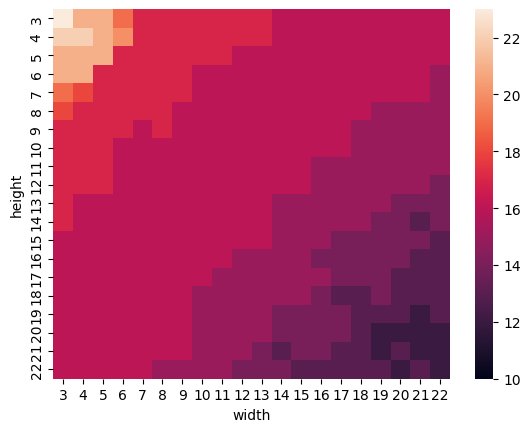
\includegraphics[width=0.8\textwidth]{figures/somhparams.png}
\caption{Hyperparameter analysis of SOM train on MSMA score-norms. The x-axis represent the width of the SOM grid, measured in number of neurons. The y-axis represents the height of the SOM grid. The heatmap shows the number of samples belonging to the Maximal-Prototype for each experiment. Note the diagonal 'stable' regions of the hyperparameter space.}
\label{fig:som-hparams}
\end{figure}

% \begin{figure}
% \centering
% \begin{subfigure}[b]{0.4\textwidth}
% \includegraphics[width=\textwidth]{figures/ds_proto–hex.png}
% \caption{A Self-Organizing Map trained on score-norms of brain MRIs of typically developing children. Overlayed are the distributions of all cohorts matched to each cell in the grid.}
% \label{fig:som-abcd}
% \end{subfigure}
% \hfill
% \begin{subfigure}[b]{0.4\textwidth}
% 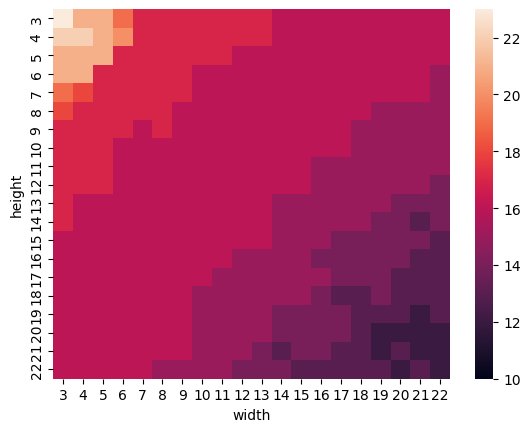
\includegraphics[width=\textwidth]{figures/somhparams.png}
% \caption{Hyperparameter analysis of SOM train on MSMA score-norms. The x-axis represent the width of the SOM grid, measured in number of neurons. The y-axis represents the height of the SOM grid. The heatmap shows the number of samples belonging to the Maximal-Prototype for each experiment. Note the diagonal 'stable' regions of the hyperparameter space.}
% \label{fig:som-hparams}
% \end{subfigure}
% \caption{SOM shows us the relative locaion of the prototypical regions in the score-norm space}
% \end{figure}


\subsection*{Prototype Consistently Detected Across Experiments}

When using a data exploration tool such as SOM for producing scientific insights, it is crucial to delineate true correlations that exist in the data and spurious correlations that may be caused by random variations in the algorithm. Therefore, to increase our confidence in the findings, it is helpful to analyze the stability of the algorithm across runs with different hyperparameters. If the algorithm outputs consistent results, then one can have more confidence when interpreting the results. Note that as we are using PCA initialization, and thus each SOM experiment is deterministic and reproducible (given the same training set).

SOM has two main hyperparameters: the number of rows, and the number of columns in the grid. We can assess whether SOM consistently finds the same Maximal-Prototype for DS. 
\figref{fig:som-hparams} shows a heatmap of the number of samples that matched the Maximal-Prototype in each experiment. We can observe that the number of matches remains consistent across different hyperparameters. Smaller grid sizes will have the most matches as there are only a few candidate prototypes. Large grid sizes will cause a more refined binning, resulting in multiple prototypes that are relatively close to one another. We can observe large ''bands" of stability in the middle regions.

Further analysis revealed that each band captures the \textit{same} samples as well as having a perfect overlap with the one before it. For instance, the set of experiments that produced a 16-sample prototype not only captured the same 16 samples within the set of experiments but also the same samples that were captured by the 15-sample prototype. This indicates that SOM is capturing a true sub-population of DS samples in the score-norm space rather than clustering at random.



% Another interesting point to note, is the specificity of this prototype. Only 17 (non-inlier) samples matched with this prototype

\subsection*{Does Spatial-MSMA Capture Relevant Brain Regions?}

\begin{figure}[tbhp]
\centering
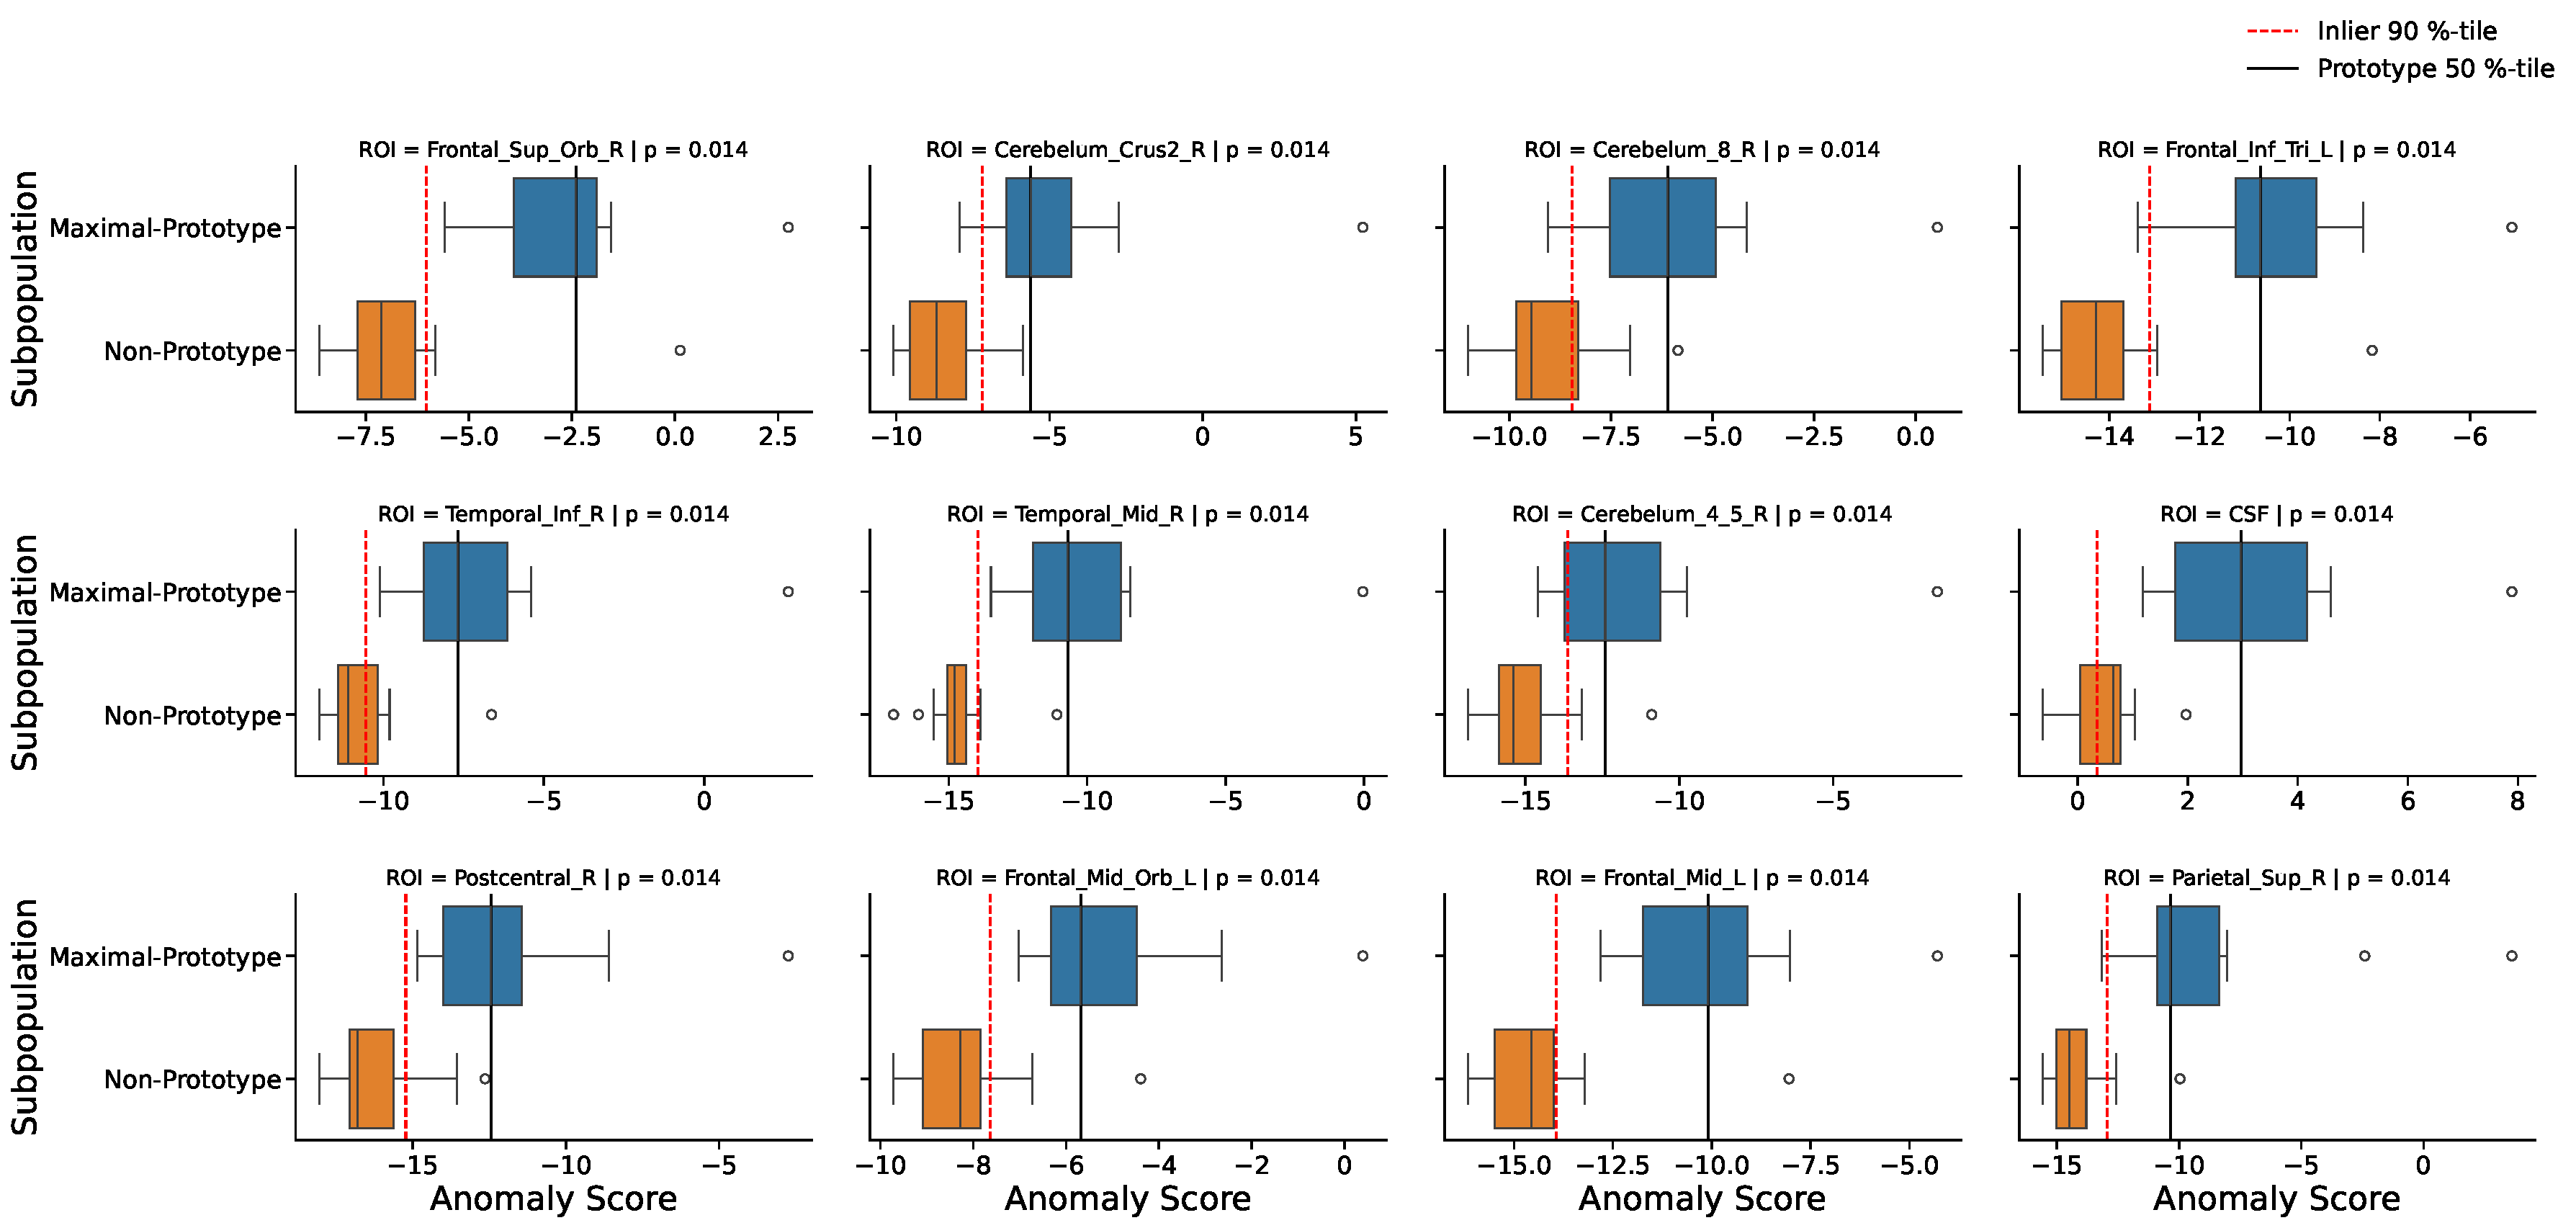
\includegraphics[width=\textwidth]{figures/roi_boxplot.pdf}
\caption{Box-Whisker plots of the most significant ROIs that significantly differ between the prototypical DS and non-prototypical DS population. The x-axis represents the anomaly score for each sample. \textit{Higher} values are more anomalous. For reference, the 90-th percentile of the inlier anomaly scores for the given ROI is also plotted (red dashed line). All plotted ROI anomaly scores have statistically significant differences in their medians after Bonferroni correction. }
\label{fig:roi-box-ds}
\end{figure}


Once a sub-population of the DS cohort is identified, we can begin to explore the brain regions that significantly differ from the rest.  This analysis will use the anomaly scores produced by Spatial-MSMA to quantify the relevance of each region. The goal of the analysis is to determine whether there are regions that are significantly different between the prototype and non-prototype populations. To select anomalous ROIs, the anomaly scores (per region/ROI) were averaged across the DS cohort. Only those regions that had an average above the 90-th percentile with respect to the \textit{inlier} population were retained for the significance analysis.

The filtered set of anomalous ROIs was used to determine whether there exists a distributional shift between the anomaly scores for the prototypical and the non-prototypical samples. Concretely, we will be using the Mann-Whitney U-test; a non-parametric test to compare the medians between two groups. This test is well-suited for our scenario as we do not have a large sample size (16 prototypical, 12 non-prototypical), and thus we cannot expect our populations to follow a Normal distribution. The null hypothesis of this test is that the two groups have the same median, and thus belong to the same underlying distribution. The p-value from the Mann-Whitney U-test represents the probability of observing a test statistic as extreme (or more extreme) as the one calculated, given that the null hypothesis is true. As this analysis will be performing a statistical test for each ROI, it is important to control for the \textit{multiple comparison problem}. One effective method is to correct for the False Discovery Rate (FDR). This correction will adjust the p-values belonging to a set of statistical tests such that a chosen significance level also corresponds to the expected proportion of false positives after thresholding. For instance, if we choose a p-value threshold of $0.01$ after FDR correction, then we can expect 1\% of the significant ROIs to be false positives. This analysis used the Benjamini-Hochberg procedure~\cite{benjamini1995controlling} for controlling FDR.


After the first stage filtering, 71 ROIs were identified. The medians of the filtered ROIs were compared across the prototypical and non-prototypical sub-populations.~\figref{fig:roi-box-full-ds} shows the 40 out of the 71 filtered ROIs that were significantly different between the prototypical samples and non-prototypical samples. The significance level was chosen to be a p-value of $0.05$, \textit{after} Bonferroni correction.

% This implies an expected FDR of \textit{only} $0.5\%$. 
\figref{fig:roi-box-ds} shows a subset of the  most significant ROIs (top 12). For reference, the $90$-percentile of the low-risk typical population is also plotted. Note how the median of the Maximal-Prototype are always higher than the 90-th percentile, whereas the same does not hold for the non-prototypes. This tells us that the model finds this subpopulation particularly anomalous.



\begin{figure}[htbp!]
\centering
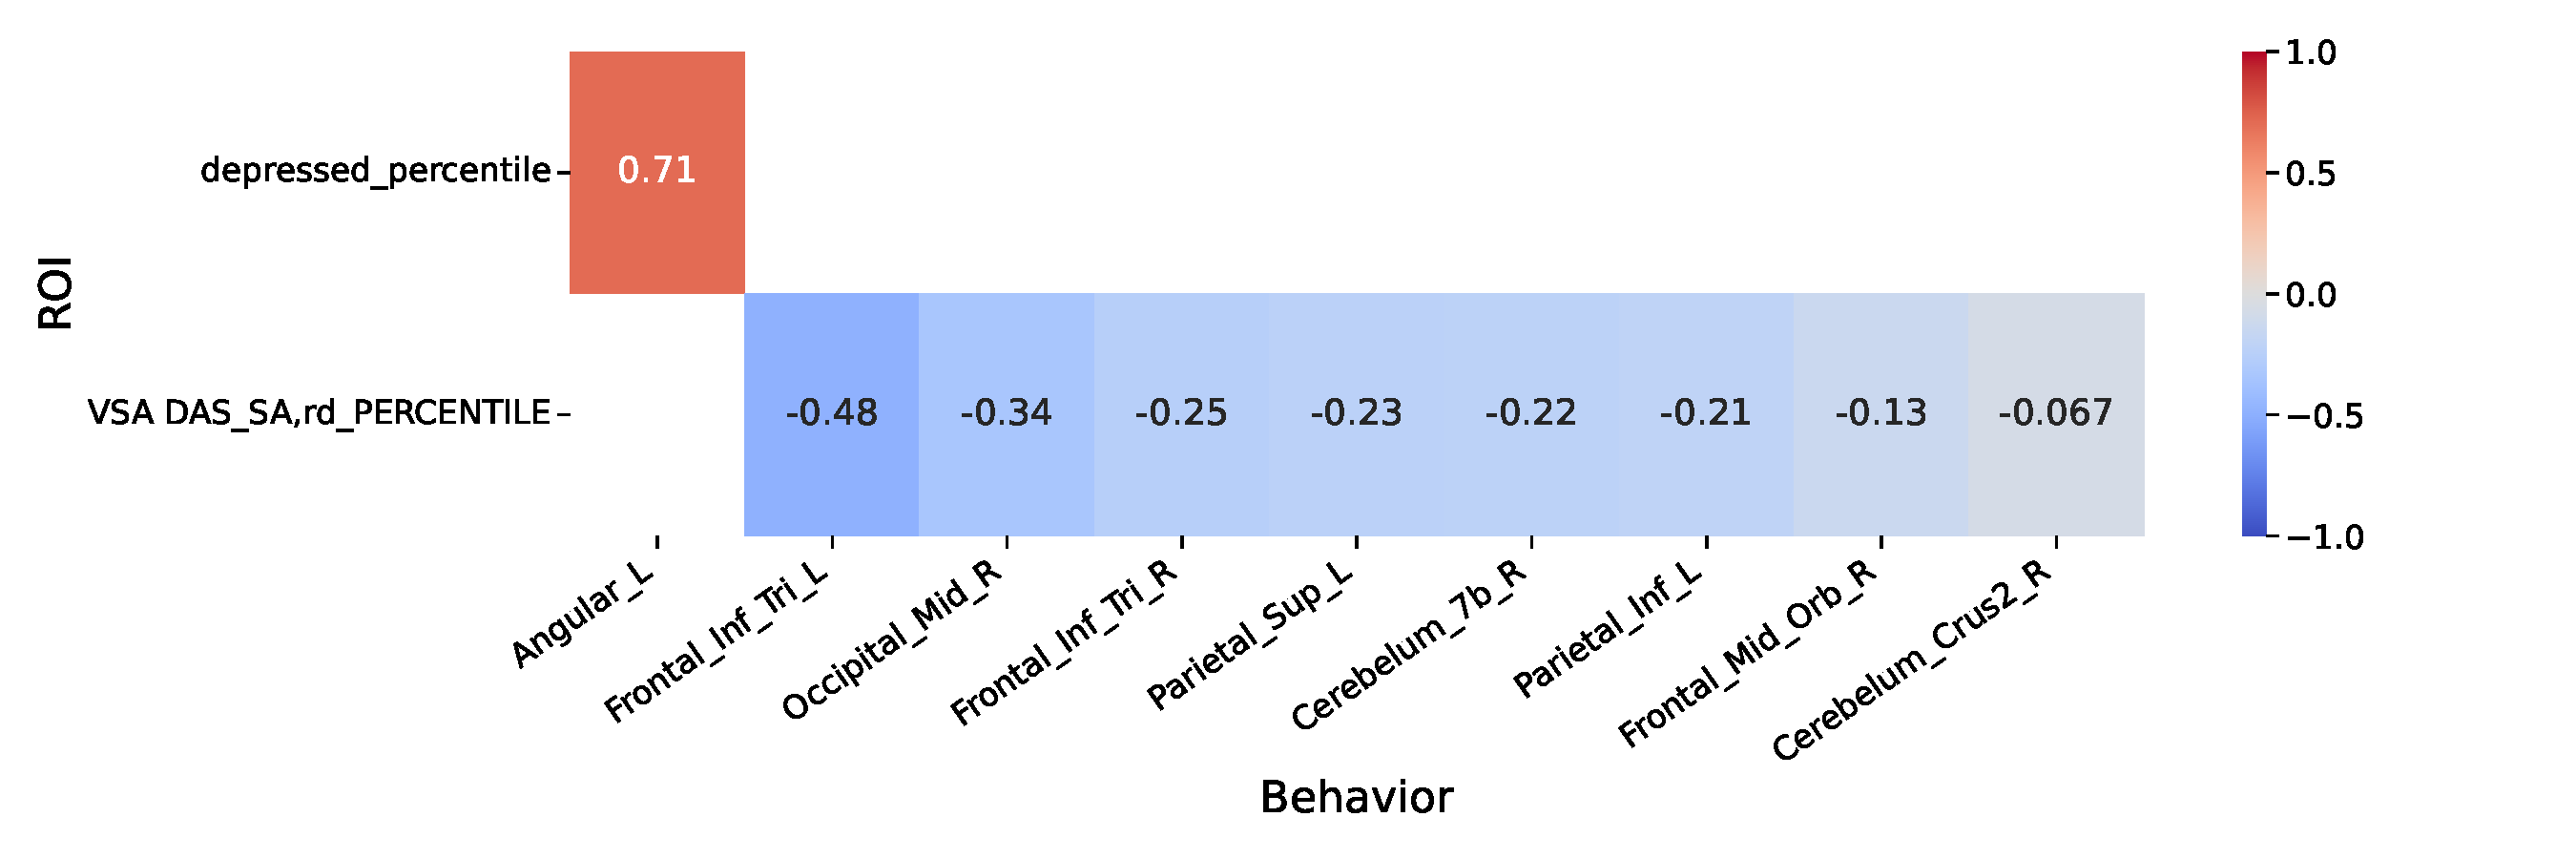
\includegraphics[width=\linewidth]{figures/sig_roi_corrs.pdf}
\caption{Heatmap of correlations between behavioral scores and ROI anomaly scores. The ROIs included in these experiments were those that were identified as significantly relevant for the prototypical class. All correlations shown are below a FDR-corrected p-value of $0.1$. Note the high correlations between certain subscores and the ROI anomaly scores. 
%We may expect 10\% of the identified pairs to be false positives.
}
\label{fig:sig-roi-corr}
\end{figure}

\subsection*{Do the regional anomaly scores correlate with behavioral assessments?}

The previous section identified a set of anomalous brain regions that significantly deviated from the non-prototypical DS samples. This section will explore whether the anomaly scores of the identified ROIs have meaningful correlations with ground truth data. Individuals with neurodevelopmental disorders often exhibit atypical behaviors compared to a typically developing cohort. These behavioral atypicalities can be captured by behavioral assessments such as CBCL and DAS (Differential Ability Scales). We can test to see whether the anomaly scores produced by Spatial-MSMA correlate with scores of such assessments. 



For each ROI, a Spearman-rank correlation was computed against a set of behavior scores. Specifically, the analysis covers CBCL, Vineland, and DAS scores. Both global, and subscores were included.
A total of 35 behavior scores and 40 ROIs were tested, resulting in 1400 correlation experiments. p-values were computed for the pairs using a Permutation test with $10,000$ permutations. An FDR correction was applied to the resulting p-values using the Benjamini-Hochberg procedure. ~\figref{fig:full-roi-corr} shows the correlation matrix for all  ROI-Behavior pairs while~\figref{fig:sig-roi-corr} shows correlations for only the significant pairs ($\text{corrected-}p < 0.1$) at an FDR of $10\%$. Specifically, the DAS subscore \textit{Recall of design} has weak to moderate negative correlations with a large number of ROIs, while the CBCL subscore \textit{depressed} has a strong correlation with the \textit{Left Angular gyrus}. 

~\figref{fig:roi-scatter} shows the linear regression plot of the ROI anomaly scores and behavioral assessment subscores (percentiles). Note that the $r$ values in the plots are the rank correlations. All pairs have \textit{corrected} p-value below $0.1$. Recall, that this implies an expected FDR of $10\%$. The plots show above moderate correlations across most ROI-Behavior pairs.

\begin{figure}[h!]
\centering
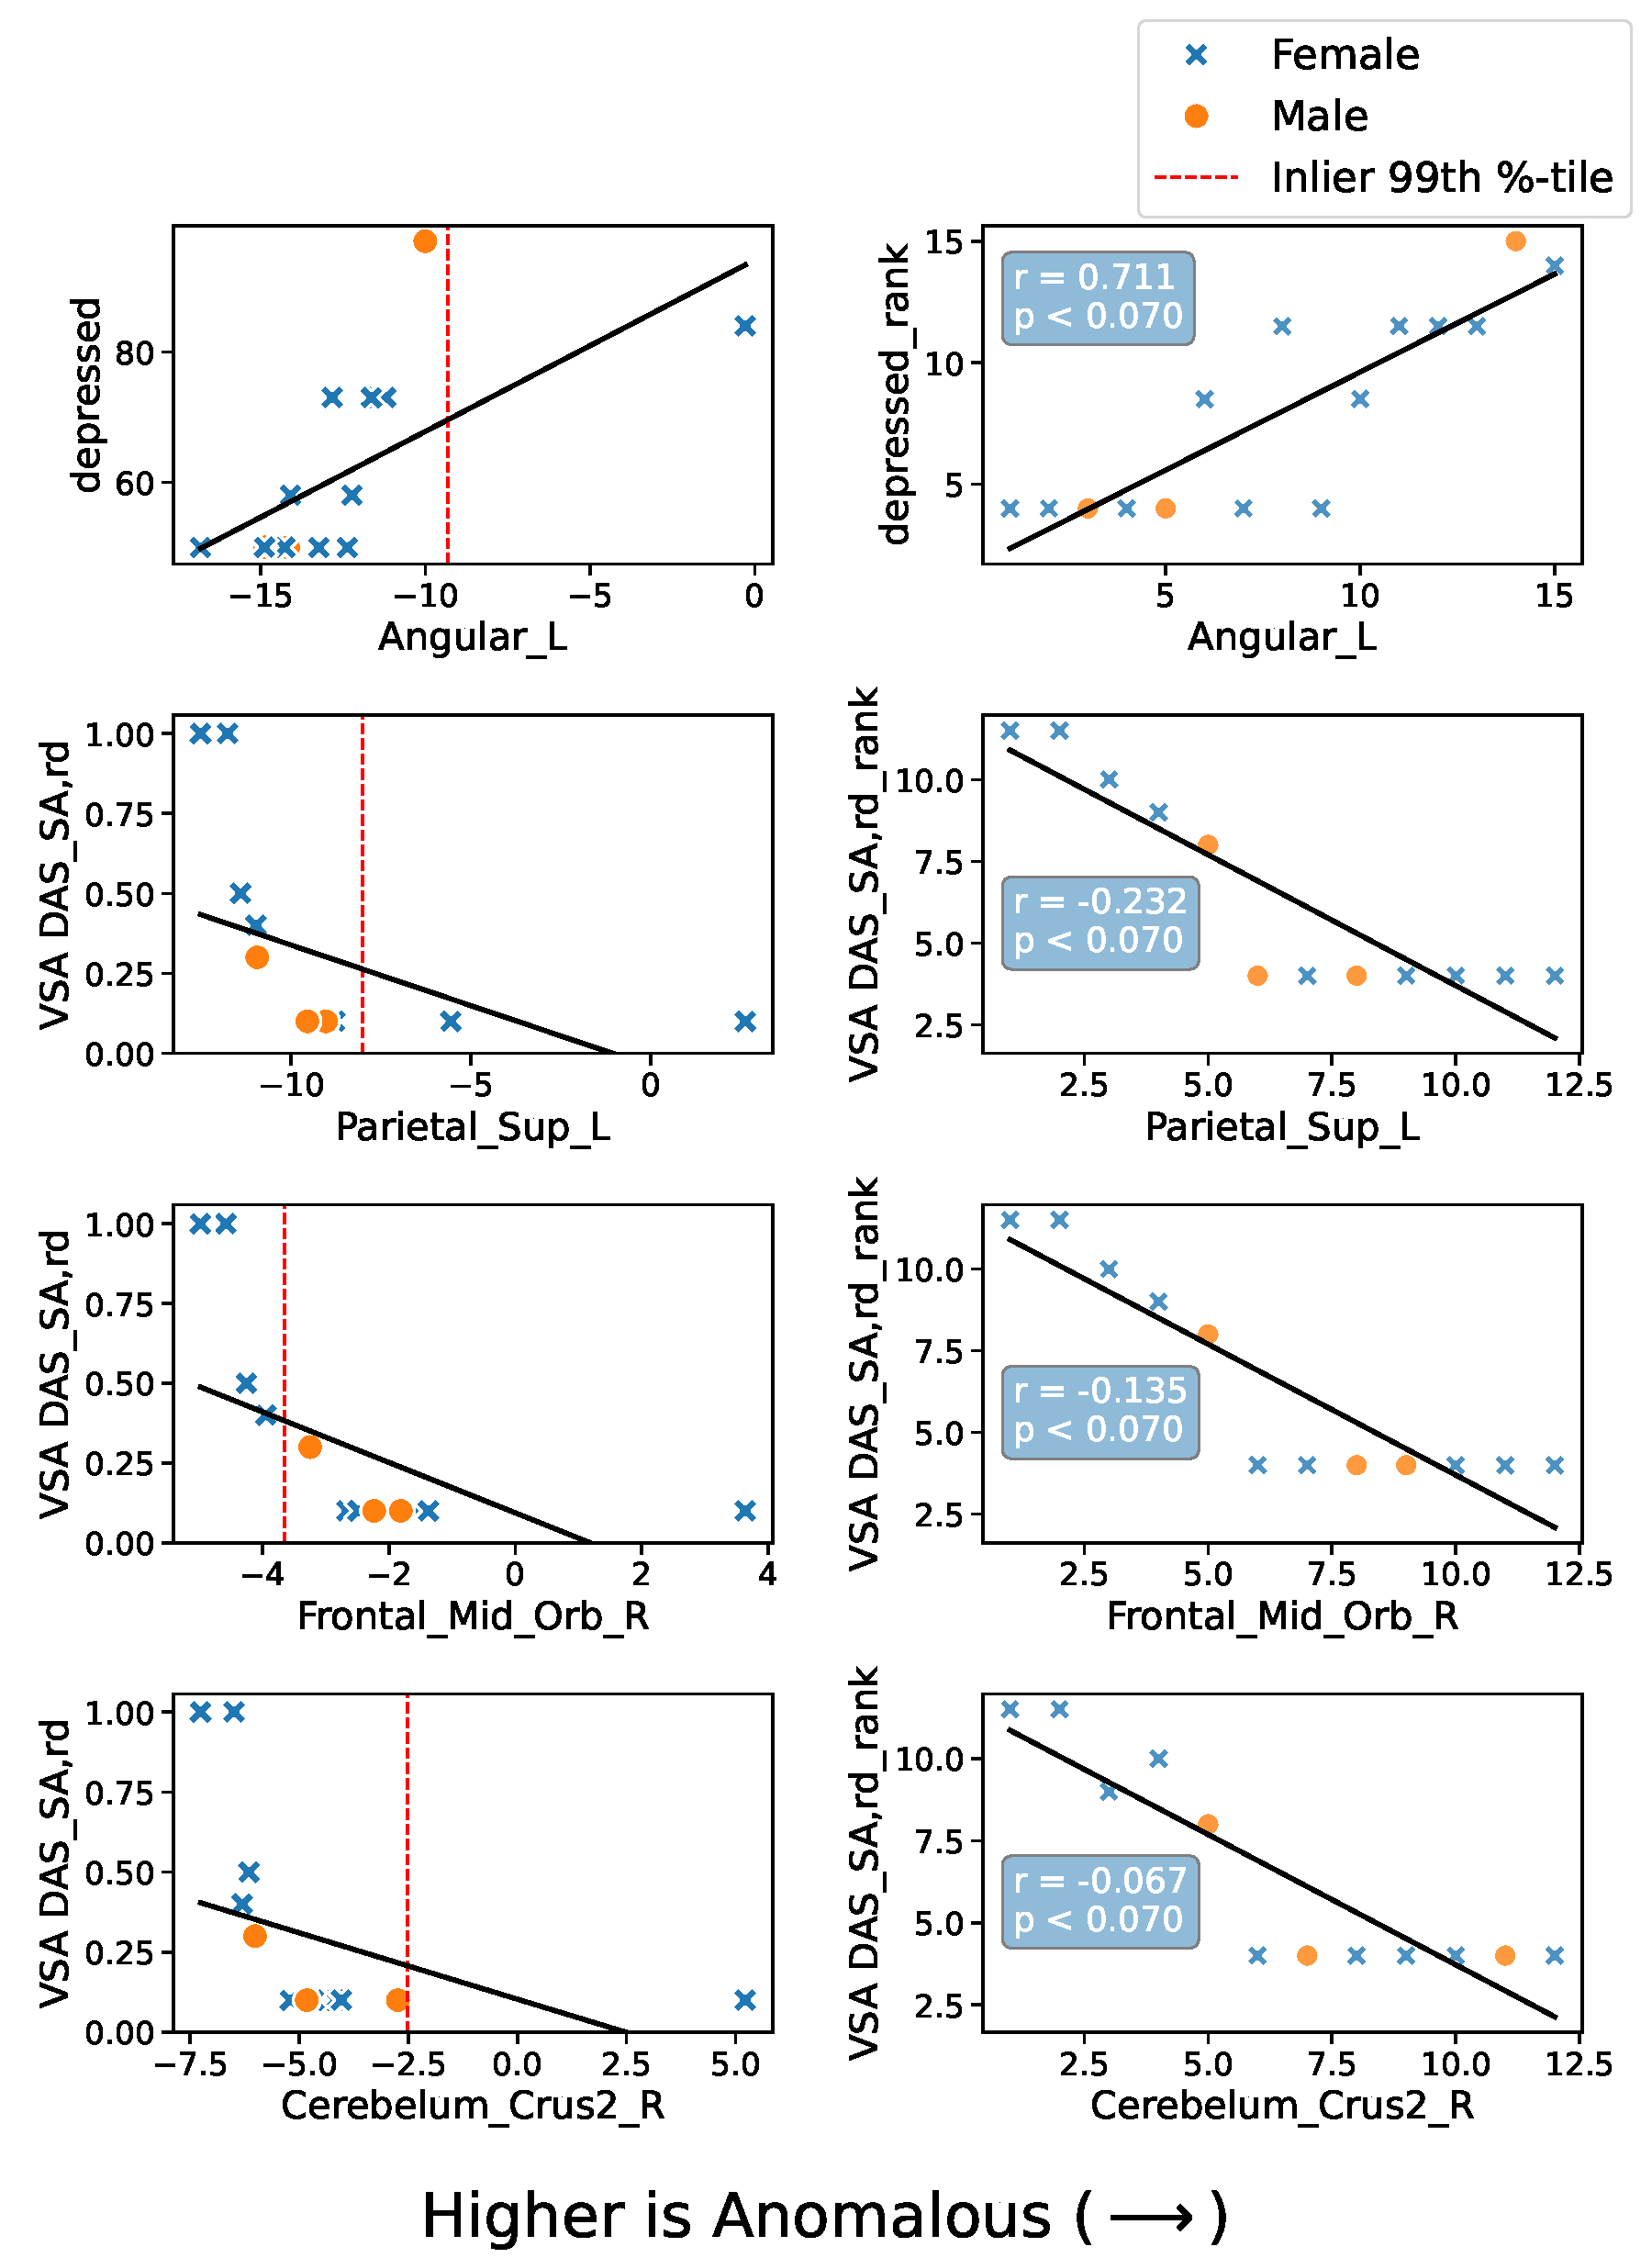
\includegraphics[width=\textwidth]{figures/rankcorrplot-fig1.pdf}
\caption{Spearman-rank correlations ($\text{corrected-}p < 0.1$) between ROIs belonging to prototypical Down Syndrome samples and behavioral scores.
First column shows raw scores (percentiles for behavior scores and negative log-likelihoods for anomaly scores), while second column shows ranks. Note that all \textit{percentiles} in the range 0-100. All p-values were corrected for FDR.}
\label{fig:roi-scatter}
\end{figure}

\begin{figure}[h!]
\centering
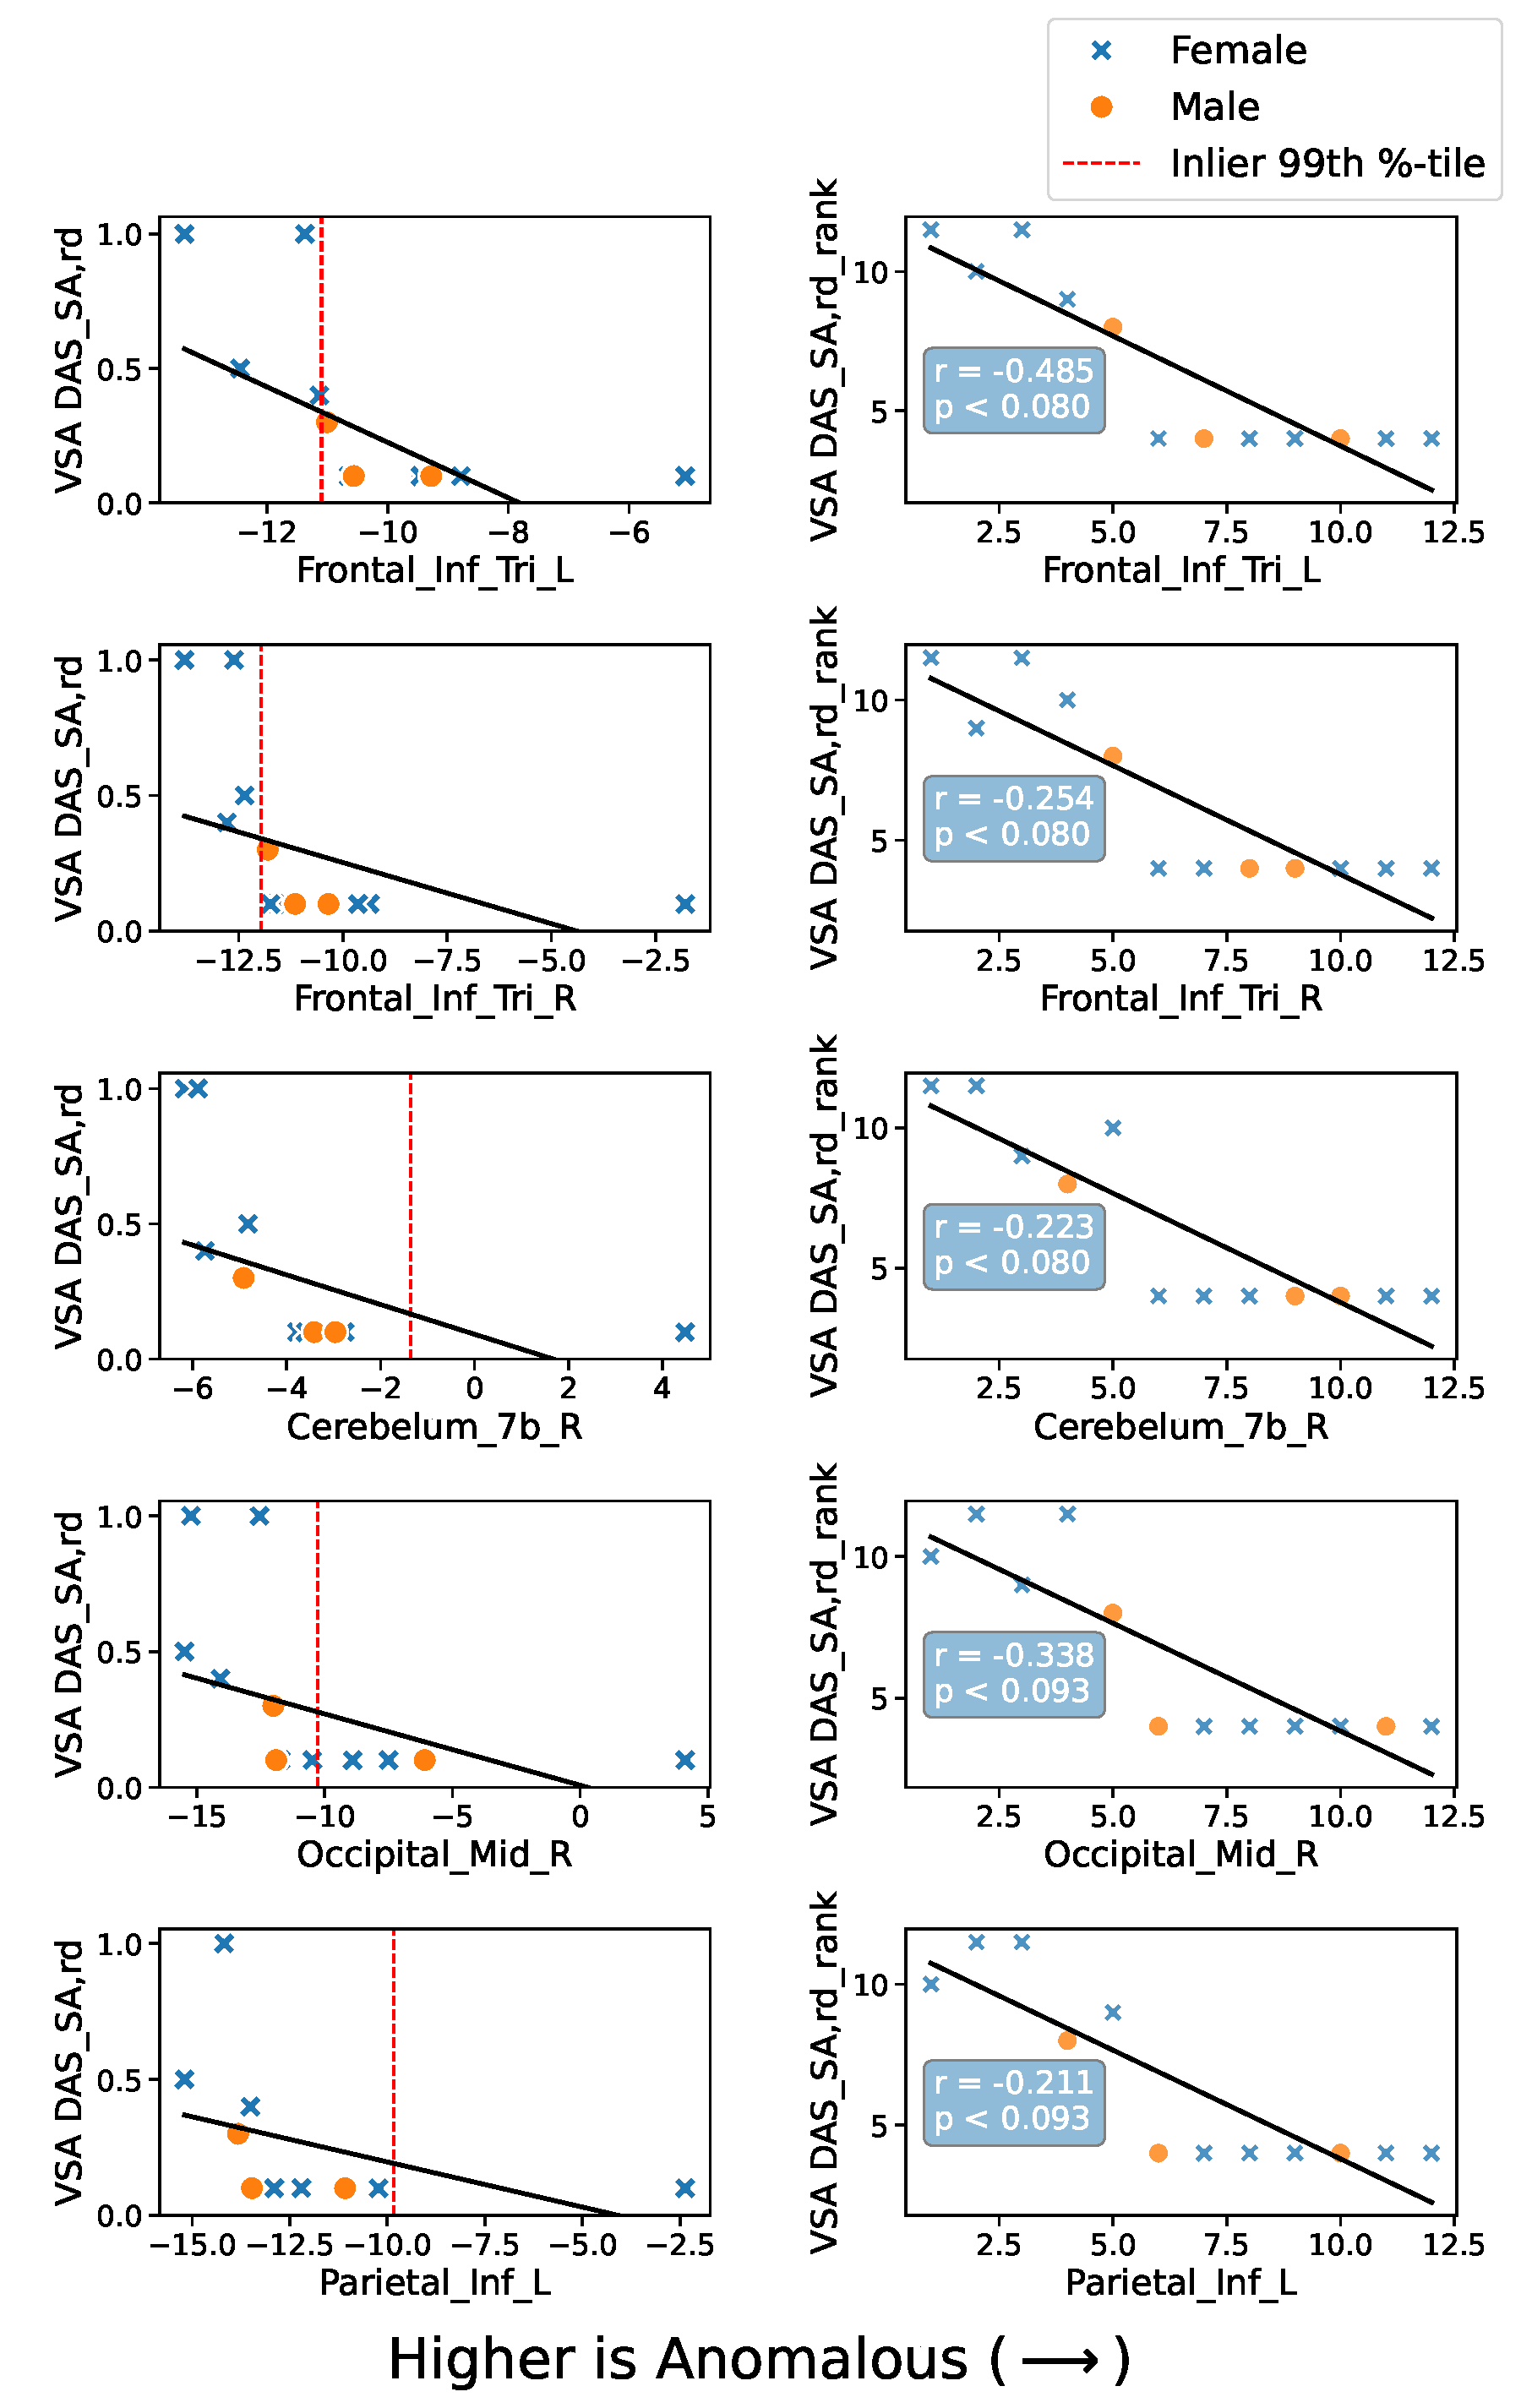
\includegraphics[width=0.93\textwidth, height=1.46\textwidth]{figures/rankcorrplot-fig2.pdf}
\caption{Continuation of correlations from~\figref{fig:roi-scatter}}
\label{fig:roi-scatter-cont}
\end{figure}


\begin{figure}[ht]
\centering
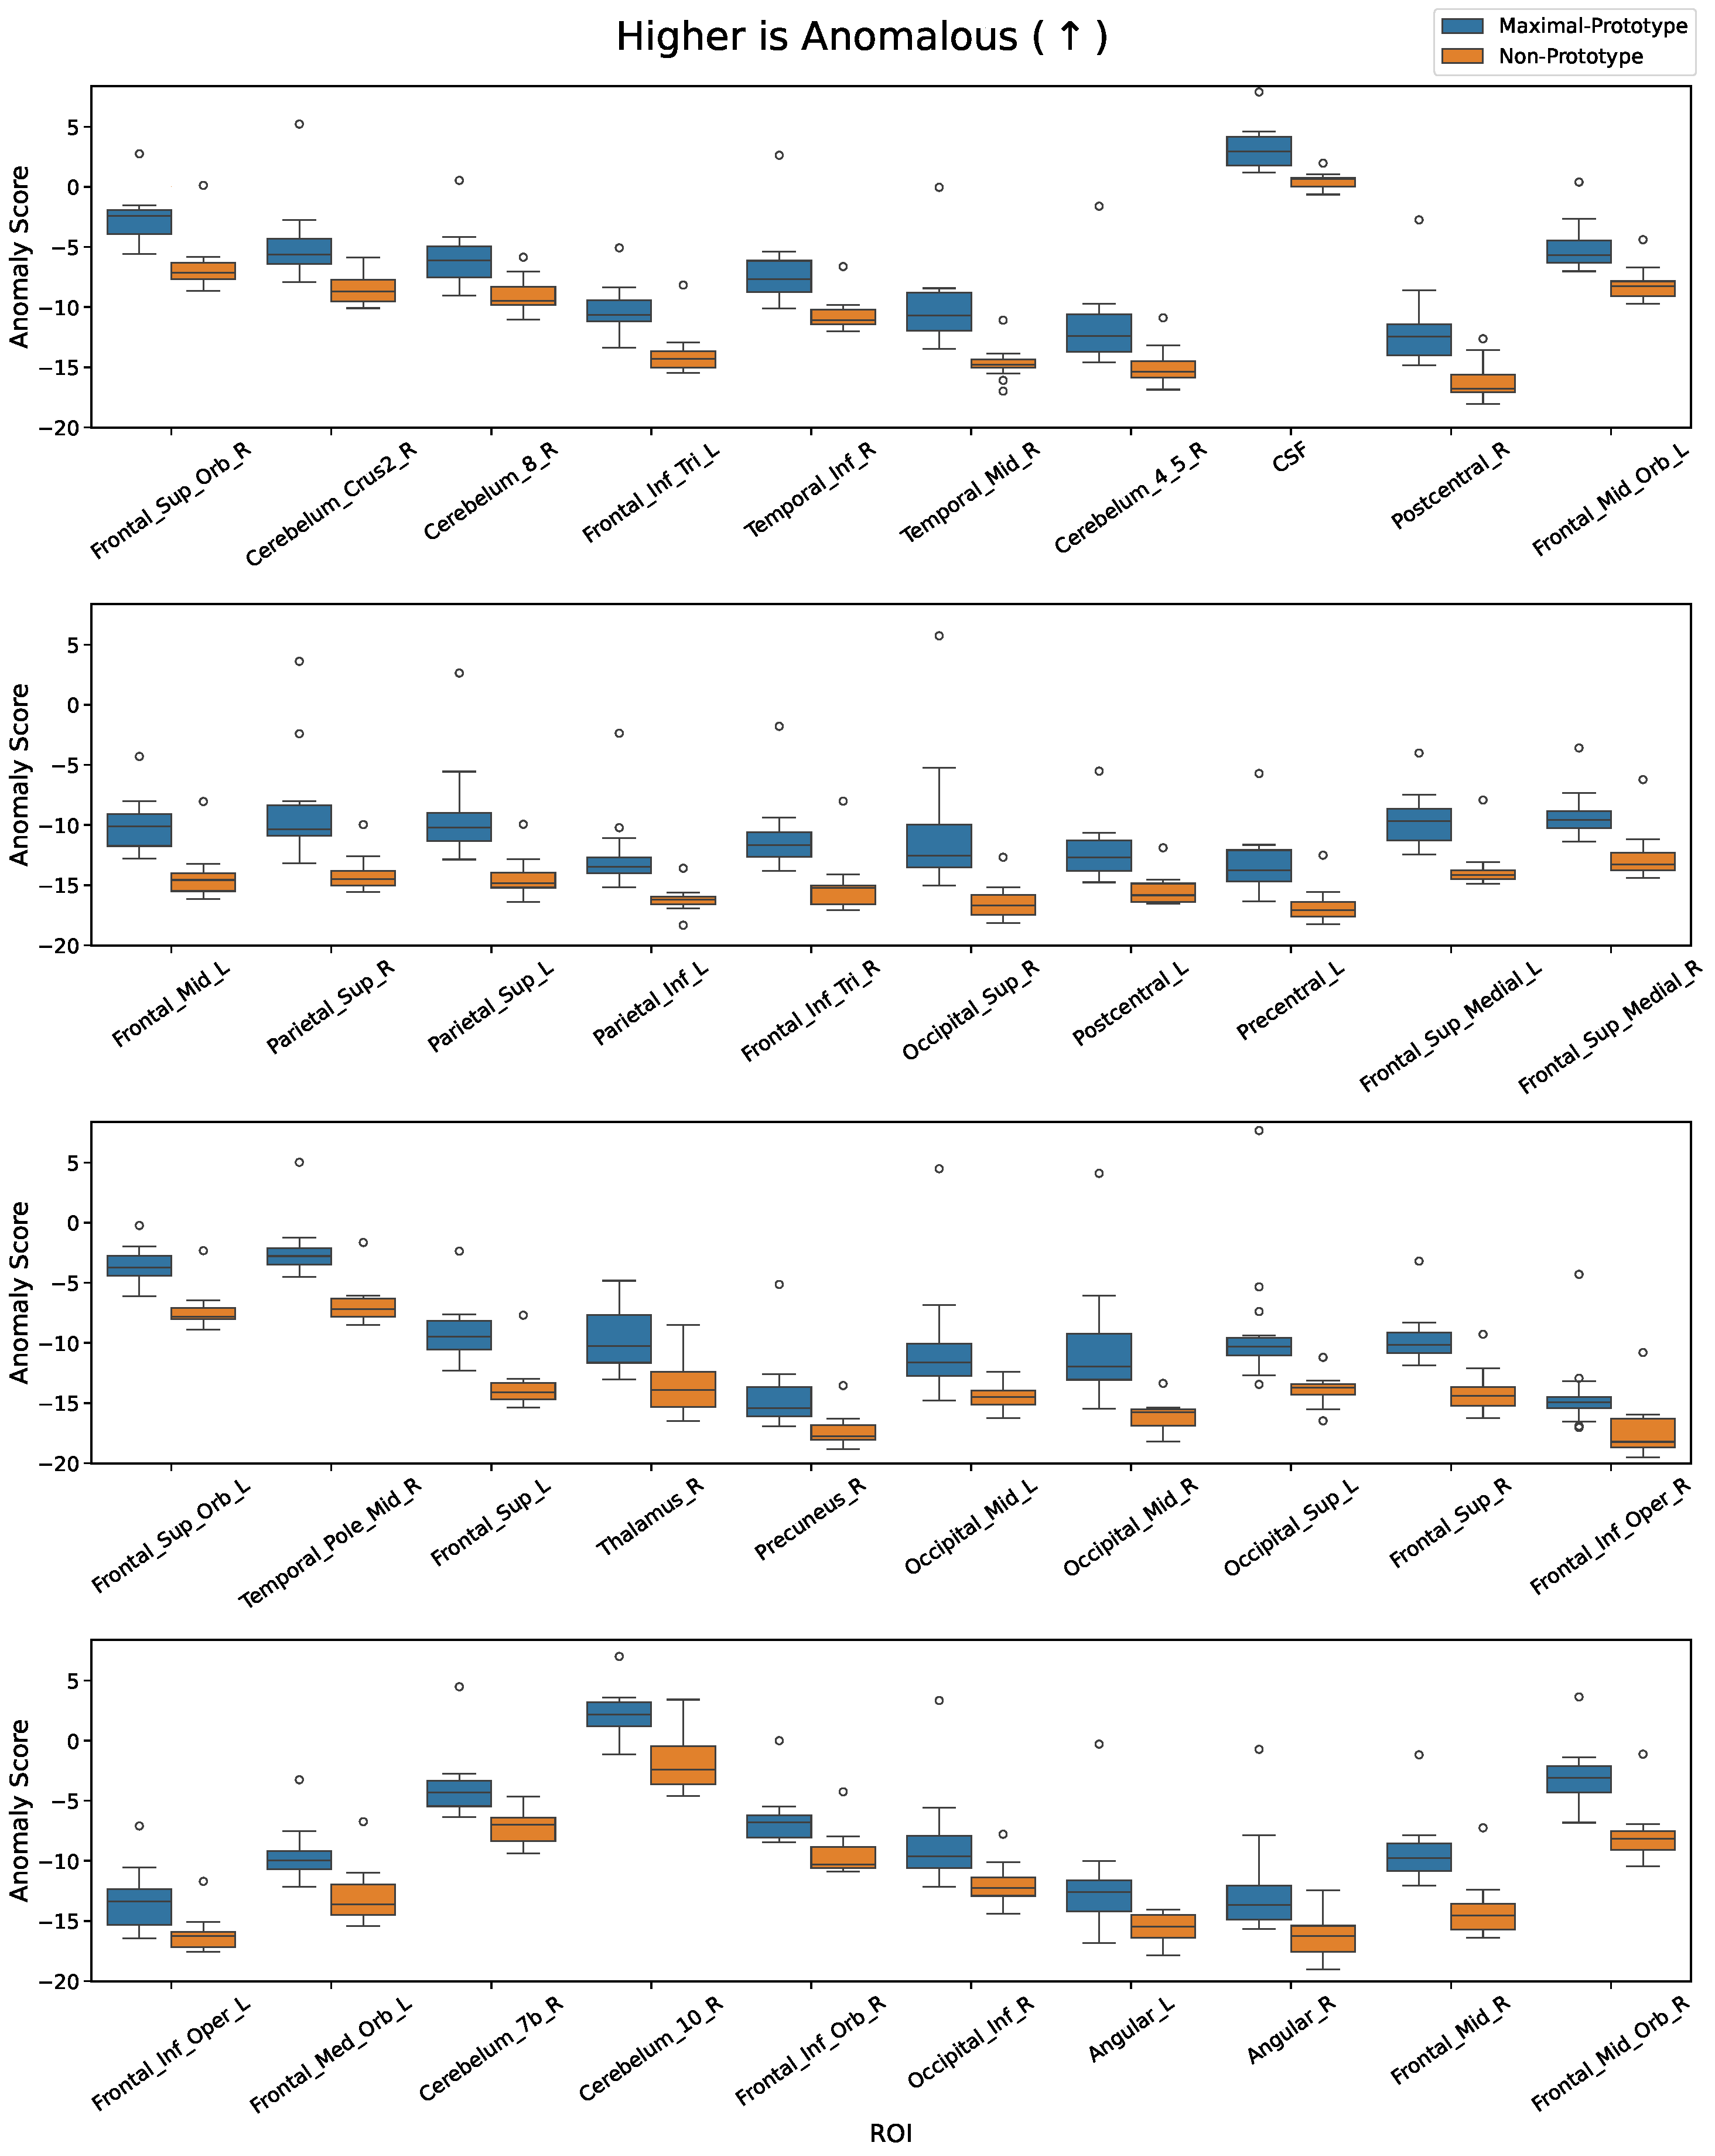
\includegraphics[width=\textwidth]{figures/roi_full_boxplot.pdf}
\caption{Box-Whisker plots of all ROIs that significantly differ between the prototypical DS and non-prototypical DS population. The ROIs are plotted in order of significance (from lower p-values to higher).  They-axis represents the anomaly score per sample, higher values indicating the presence of higher anomalies. All plotted ROI anomaly scores have statistically significant differences in their medians \textit{after} Bonferroni correction ($p < 0.05$). }
\label{fig:roi-box-full-ds}
\end{figure}




\begin{figure}[tbhp]
\centering
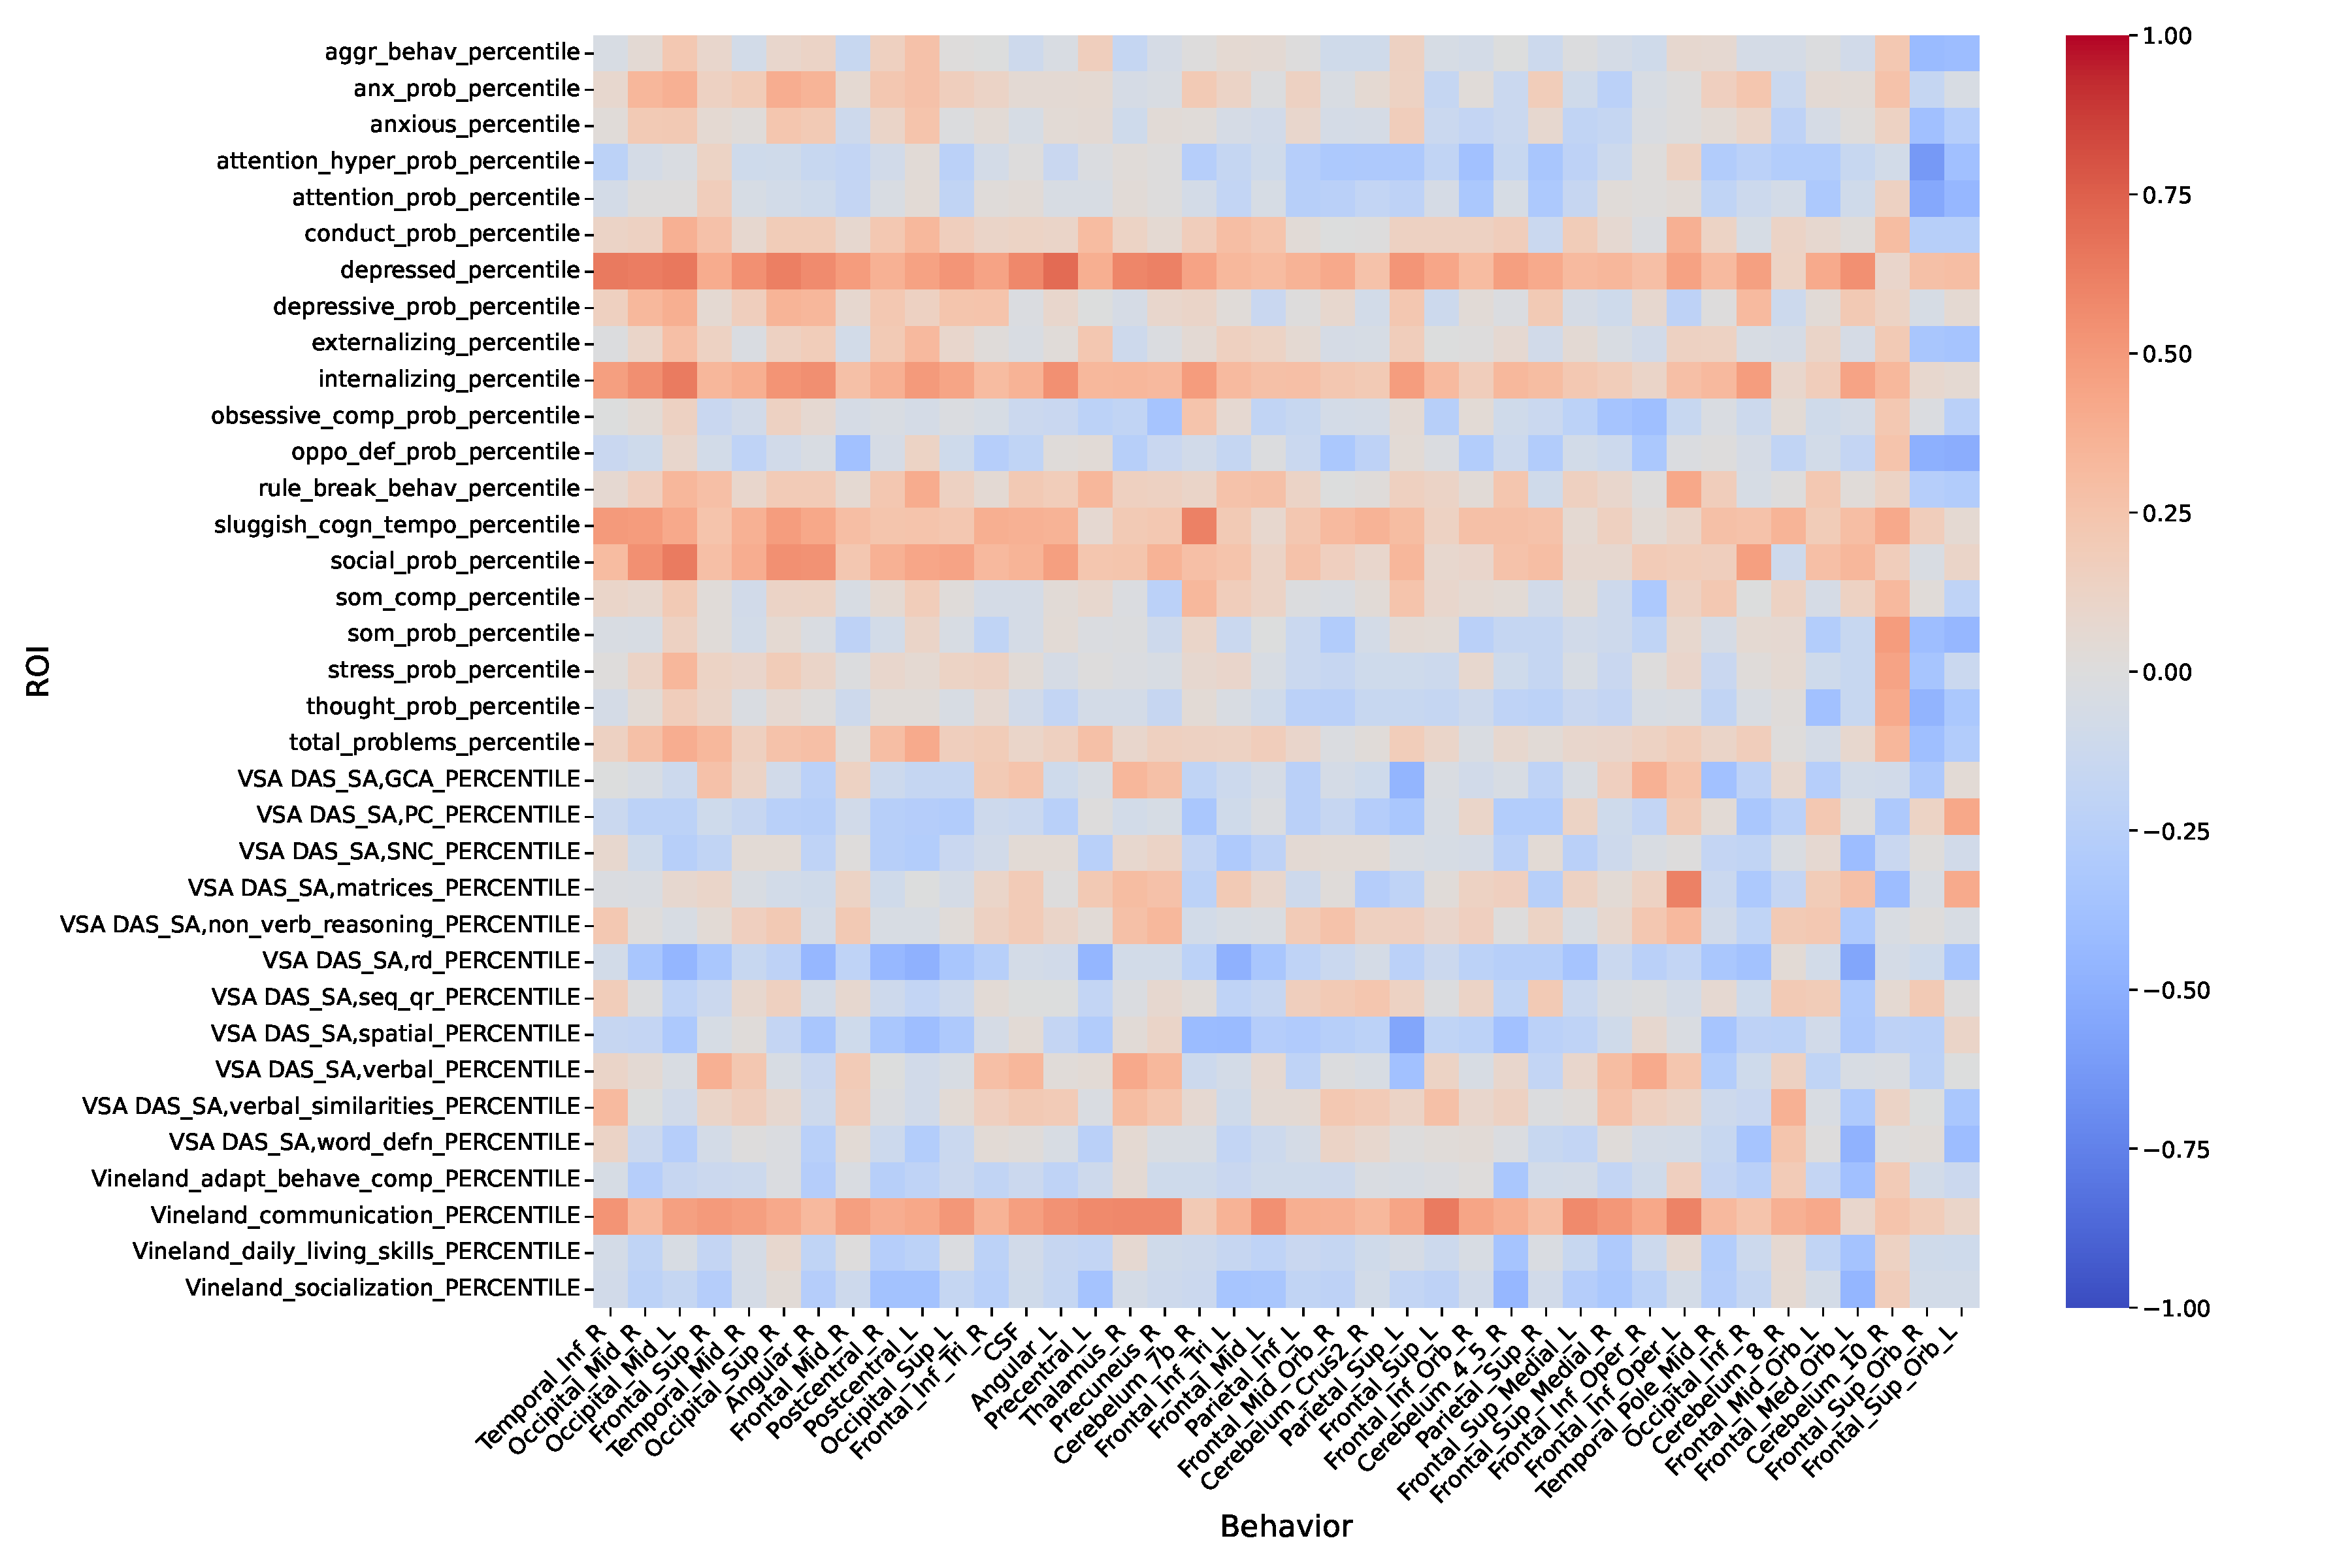
\includegraphics[width=\linewidth]{figures/full_corrmatrix.pdf}
\caption{Heatmap of Spearman-rank correlations between behavioral scores and ROI anomaly scores. Most of these correlations are not significant after FDR correction due to the low sample size.}
\label{fig:full-roi-corr}
\end{figure}

\begin{figure}[tbhp]
\centering
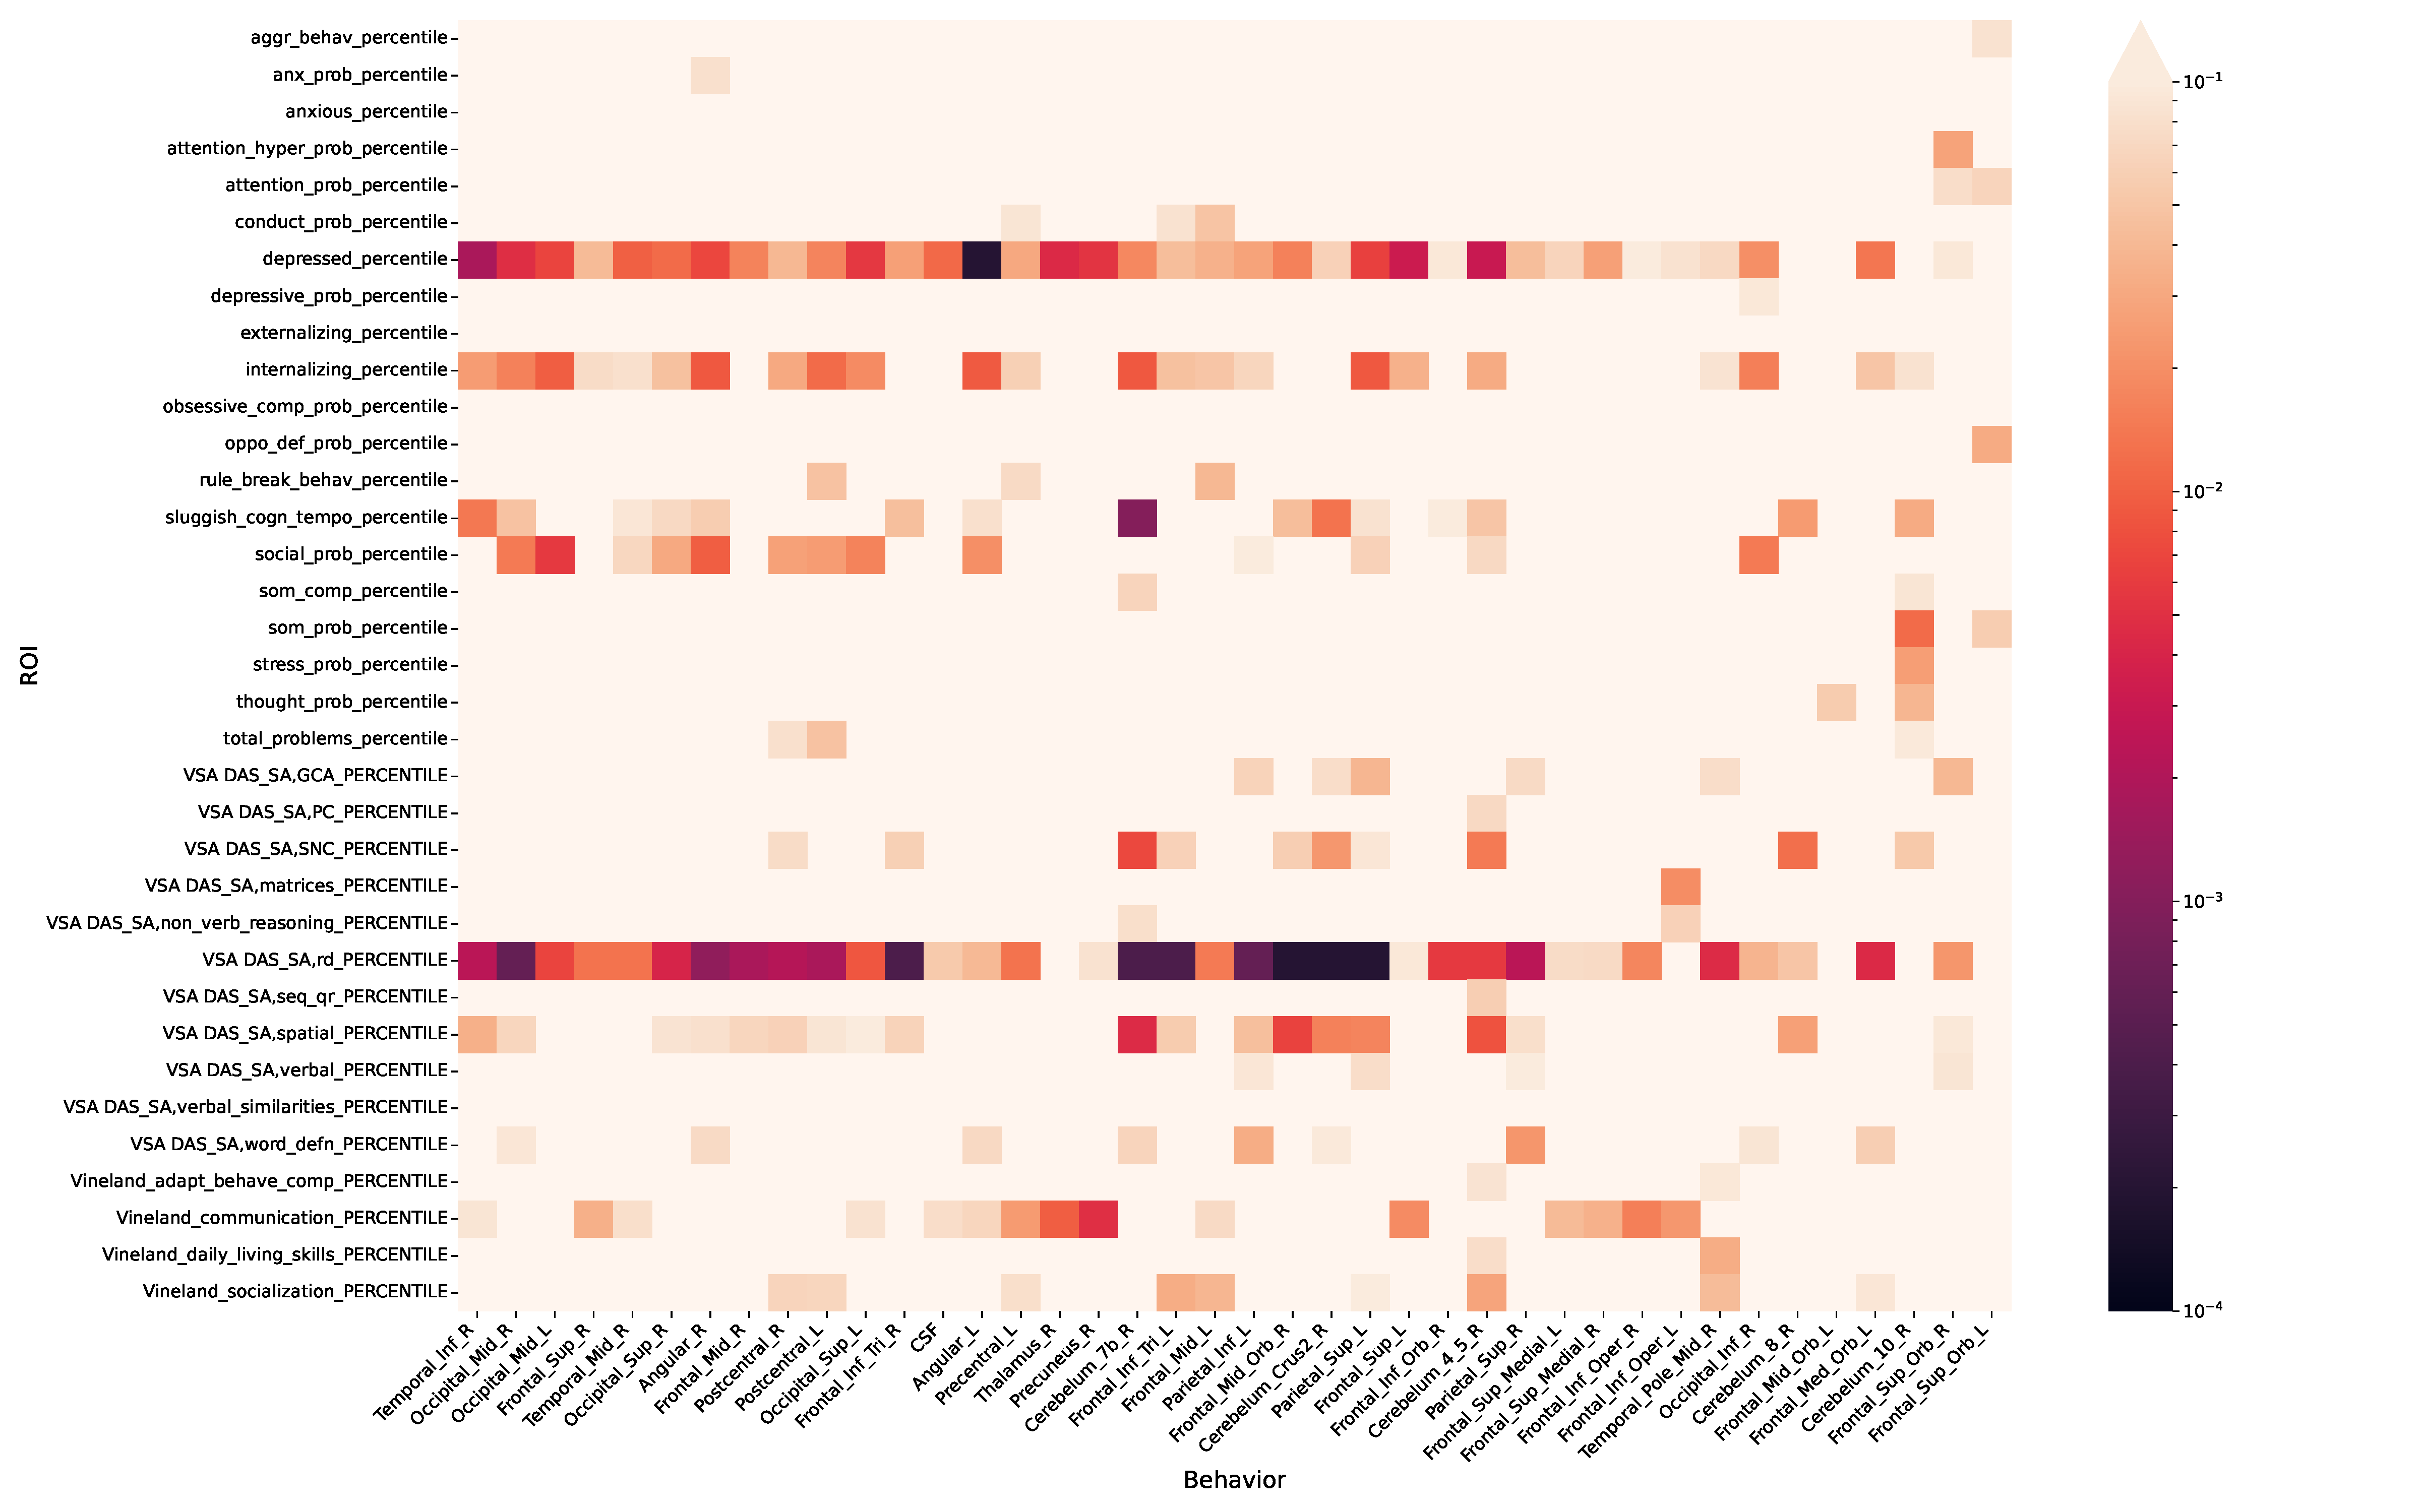
\includegraphics[width=\linewidth]{figures/pmatrix.pdf}
\caption{Heatmap of raw p-values for tested Behavioral-ROI correlation tests. Only showing $p < 0.1$.}
\label{fig:full-roi-corr}
\end{figure}

\section{Conclusion}

This chapter has demonstrated the potential for using the score-based representations learned by MSMA to gain valuable scientific insights, rather than just using them for anomaly detection. By leveraging the SOM algorithm to visualize the score-norm space, we were able to identify a distinct subpopulation within the Down Syndrome cohort that exhibited a characteristic neuroanatomical phenotype. The stability of this prototypical pattern across different SOM hyperparameter settings provided confidence that it represents a true underlying pattern in the data, rather than an artifact of the visualization technique.

Further analysis using Spatial-MSMA localized this prototypical pattern to specific brain regions that were significantly different from the non-prototypical Down Syndrome samples. Importantly, these identified brain regions were found to strongly correlate with behavioral measures like the CBCL, and Vineland assessments. This suggests that score-based representations are capturing meaningful neuroanatomic features that are linked to the functional and behavioral manifestations of Down Syndrome.

Overall, the case-study presented in this chapter showcases how the combination of MSMA, and Spatial-MSMA can be a powerful framework for not just detecting anomalies, but also generating substantive scientific hypotheses about the underlying drivers of atypical neurodevelopment. By connecting anomalous brain features to validated behavioral assessments, this methodology provides a data-driven approach to uncover the neuroanatomical basis of neurodevelopmental disorders. Future work can further expand on these insights to inform targeted neuroimaging biomarkers and intervention strategies.